\chapter{Introduction}
\label{chapter:Introduction}

Well, you are about to write your thesis? There is no need to tell you that there are several months of hard work ahead. However, we try to support you by providing this \LaTeX\ template, which is hopefully easy to use and needs only little explanation. This chapter is meant to help you to set up a project for your written thesis. Moreover, there are examples for frequent content such as, for instance, figures, listings, and references to literature as well as online resources.

%*********************************************************************************
%---------------------------------------------------------------------------------
\section{Getting Started with this Template}
%---------------------------------------------------------------------------------
%*********************************************************************************

Please start your journey by editing the main file \emph{Thesis.tex} in the root directory. The file contains a section where you specify basic information (e.~g., your name and degree course, the examiners, title of the thesis), layout settings, and the files containing your chapters and appendix. Most settings are described by comments in \emph{Thesis.tex} and should be self-explanatory. Still, let us give you some further information.

%---------------------------------------------------------------------------------

\paragraph{Language} Please specify the language you use for your written thesis as either German (\emph{DE}) or English (\emph{EN}). This setting must match the language of the officially registered title, but need not match the prevailing language used in lectures of your degree course. For instance, a student of the degree course \emph{B.Sc. Elektrotechnik und Informationstechnik} may write a thesis in English.
%
\begin{lstlisting}[language=bash]
\Language{EN}
\end{lstlisting}

%---------------------------------------------------------------------------------

\paragraph{Degree course} Specify your degree course using one of the abbreviations listed in the respective comment in \emph{Thesis.tex} (e.~g., \emph{IE} for \emph{B.Sc. Information Engineering}).
%
\begin{lstlisting}[language=bash]
\DegreeCourse{IE}
\end{lstlisting}

%---------------------------------------------------------------------------------

\paragraph{None-disclosure} Set the value \emph{Confidential} to 1, if and only if your thesis must not be published. This is typically the case for theses written at a company.
%
\begin{lstlisting}[language=bash]
\Confidential{0}
\end{lstlisting}

%---------------------------------------------------------------------------------

\paragraph{Single-sided or double-sided} Set \emph{SingleSidedPrint} to 1 or 0 to generate a PDF for single-sided or double-sided printing, respectively. Many examiners prefer single-sided documents, because they can use the empty pages at the left of their printed copy for comments and corrections. However, obviously double-sided printing reduces the number of physical sheets of paper. It may be a good idea to align with your examiners before switching to double-sided printing.
%
\begin{lstlisting}[language=bash]
\SingleSidedPrint{1}
\end{lstlisting}

%---------------------------------------------------------------------------------

\paragraph{Title's font size} Typically, it looks strange when the title on the cover page uses more than two or three lines. You can adapt the font size by setting \emph{TitleFontSize} to \emph{large}, \emph{normal}, or \emph{small}.
%
\begin{lstlisting}[language=bash]
\TitleFontSize{normal}
\end{lstlisting}

%---------------------------------------------------------------------------------

\paragraph{Examiners} Please specify the gender of your supervisor and second examiner as either \emph{male} or \emph{female}. This setting is relevant for theses written in German, only, to print either ``Prüfer'' or ``Prüferin'' and ``Zweitgutachter'' or ``Zweitgutachterin'' on the page containing general information about the thesis.
%
\begin{lstlisting}[language=bash]
\Supervisor{Prof. Dr.-Ing. Marc Hensel}{male}
\SecondExaminer{Prof. Dr. rer. nat. Ulrike Herster}{female}
\end{lstlisting}

%---------------------------------------------------------------------------------

\paragraph{Bilingual abstract} Please note that every thesis must contain the abstract page in German \emph{and} English. Therefore, you must specify the title, keywords, and the text of the abstract in both languages.
%
\begin{lstlisting}[language=bash]
\Titles{German}{English}
\Keywords{German}{English}
\Abstracts{German}{English}
\end{lstlisting}

%---------------------------------------------------------------------------------

\paragraph{List of figures etc.} You can enable or disable lists of figures, tables, and listings by setting the respective value to 1 or 0. In case of doubt, align with your supervisor which lists to include in your thesis.
%
\begin{lstlisting}[language=bash]
\ListOfFigures{1}
\ListOfTables{1}
\ListOfListings{1}
\end{lstlisting}

%---------------------------------------------------------------------------------

\paragraph{Chapters and appendix} Specify the \LaTeX\ files containing your chapters and appendix. We recommend to store the \emph{*.tex} files in the subfolders \emph{.$\backslash$Chapters} and \emph{.$\backslash$Appendix}, respectively, and image files in corresponding subfolders of \emph{.$\backslash$Figures}. Leave the command \emph{Appendix} empty, in case your thesis does not contain an appendix.
%
\begin{lstlisting}[language=bash]
\Chapters{
	% Introduction
%
\chapter{Introduction}\label{ch:introduction}

This chapter describes the overall context of the thesis work, why nonlinearity is detrimental to navigational radar systems, and how digital predistortion is useful for combating these effects. The problem environment is then defined, and objectives of this thesis are established. 

\section{Motivation}

Marine radar is the primary sensor for situational awareness and collision avoidance at sea, particularly at night, in fog, and in heavy precipitation, when optical observation of the surroundings is unreliable or impossible. To obtain both long detection range and fine range resolution without resorting to very high peak transmit power, the \gls{ac:ssr-x} radar employs pulse compression: a long, modulated pulse is transmitted and compressed in the receiver by matched filtering, so that the achievable range resolution is set by the signal bandwidth rather than by the pulse duration. The detection performance of such a system depends directly on the energy that the transmit chain can put on the target, and thus on the power amplifier at the end of that chain.

This is where a fundamental limitation arises. A power amplifier behaves approximately linearly only well below its saturation point; as the input drive increases, gain compression and phase distortion set in, described by the amplifier's \gls{ac:am-am} and \gls{ac:am-pm} characteristics. The consequences are twofold. Spectrally, the nonlinearity produces intermodulation products and harmonics that broaden the transmitted spectrum. The International Standard IEC 62388 requires X-band maritime radar to transmit within the allocated band of 9.2--9.5\,GHz \cite[Sec.~6.2.1.1]{iec}, so such spectral regrowth places compliance at risk and may interfere with neighbouring services and other radars. In the signal domain, the distorted transmit waveform no longer matches the receiver's compression filter. The compressed pulse loses peak amplitude and, more critically, its range sidelobes rise. Elevated sidelobes around a strong target mask weaker targets in its immediate vicinity -- a small vessel, a navigation buoy, or floating debris alongside a large ship -- and, once the sidelobe level exceeds the detection threshold, they can appear as false targets on the radar image. Both outcomes directly undermine the reliability of the instrument the crew is expected to trust.

The conventional remedy is to operate the amplifier with a generous power back-off, keeping it inside its linear region. This is a costly compromise: the available output power, and with it the \gls{ac:snr} at the receiver, is deliberately left unused, and the amplifier is run at poor power efficiency. Digital predistortion offers an alternative. By applying the inverse of the amplifier's nonlinear characteristic to the signal in the digital domain before amplification, the effective transfer characteristic of the amplifier chain is linearised, allowing the amplifier to be driven closer to saturation while remaining spectrally compliant. The gain is a purely digital one and requires no additional expensive analogue hardware.

If this work produces successful results, the benefit is therefore concrete. Additional \gls{ac:snr} headroom translates into a longer detection range, or into the detection of targets with a smaller radar cross section at the same range, on hardware that already exists in the field. Reduced range sidelobes restore the ability to resolve weak targets close to strong ones and reduce the likelihood of false targets appearing on the display. For the radar developers, the work supplies a quantified understanding of how amplifier nonlinearity degrades their system and a validated means of correcting it; for the crews who navigate by the resulting radar image, it means a more trustworthy picture of their surroundings and a better chance of avoiding a collision. Thus, the work aims to improve the fidelity of the safety-critical radar navigation system without a significant rise in cost.

\section{Environment}

This thesis is carried out externally at NACOS Marine GmbH, a supplier of integrated marine navigation and radar systems, within the Radar Development Team -- responsible for the development and maintenance of the company's radar transceivers amongst other devices. Amongst the developed devices is the \gls{ac:ssr-x} radar transceiver. This device, more specifically its pulse compression signal chain, serves as the subject of the work. In the transmit chain, the medium and long baseband pulses used in the radar's standard operating mode are generated in firmware, windowed, upconverted to \gls{ac:if}, converted to the analogue domain, and finally upconverted to \gls{ac:rf} before being amplified for transmission. The echo returns attenuated and delayed and passes through the receive chain, where it is amplified, downconverted to \gls{ac:if} and to baseband, and filtered, before pulse compression is performed to maximise \gls{ac:snr} and to determine the target range from the echo delay. The power amplifier chain of the transmit path and its effect on the compressed output form the focus of this thesis. This is described in more detail in Chapter~\ref{ch:requirements_analysis}.

The \gls{ac:ssr-x} is an existing, productive platform that is actively maintained and further developed; this work does not introduce a new radar but investigates and improves a well-defined part of an established one. Its results feed into the wider effort at NACOS Marine to increase radar performance and to safeguard spectral compliance with IEC 62388. The assessment of its effect on spectral and pulse compression metrics, is a central part of this thesis. 

\section{Objectives}

The superordinate goal to which this thesis contributes is to increase the detection performance of the \gls{ac:ssr-x} pulse compression radar and to secure its spectral compliance without modifying its analogue hardware, by exploiting the amplifier headroom that nonlinearity currently makes unusable. Within this frame, the aim of this thesis is twofold: first, to understand the influence of power amplifier nonlinearity on the power amplifier chain of the \gls{ac:ssr-x} pulse compression radar, and second, to counteract these effects using digital predistortion. This aim is pursued by first developing a generic simulation to model the rough behaviour of the \gls{ac:ssr-x} pulse compression radar in software. Subsequently, the simulation will be finetuned through lab measurements on the real hardware to provide a precise model of the system and its behaviour. Finally, this simulated model will lay the groundwork for experiments on examining power amplifier nonlinearity effects and testing predistorton algorithms to counteract these. Results of these observations and experiments will be evaluated to draw definitive conclusions to enhance performance. 
	% Fundamentals
%
\chapter{Fundamentals}\label{ch:fundamentals}

This chapter covers the theoretical foundations and current state of technology essential for understanding this thesis work. The first section provides a basic introduction on what pulse compression radar is and how it generally works. The following two sections discuss the effects of nonlinearity and existing models that describe the nonlinearity exhibited by power amplifiers. Finally, predistortion is discussed - namely the general concept, how it can compensate for nonlinearity effects, and prominent predistortion algorithms in practice.

The goal of this chapter is not to cover the entire field of radar theory and nonlinearity at large, but rather to cover the key concepts and theory directly pertinent to this thesis work. This provides the reader context and prior knowledge to comprehend the work. 

\begin{figure}[tb]
  \centering
  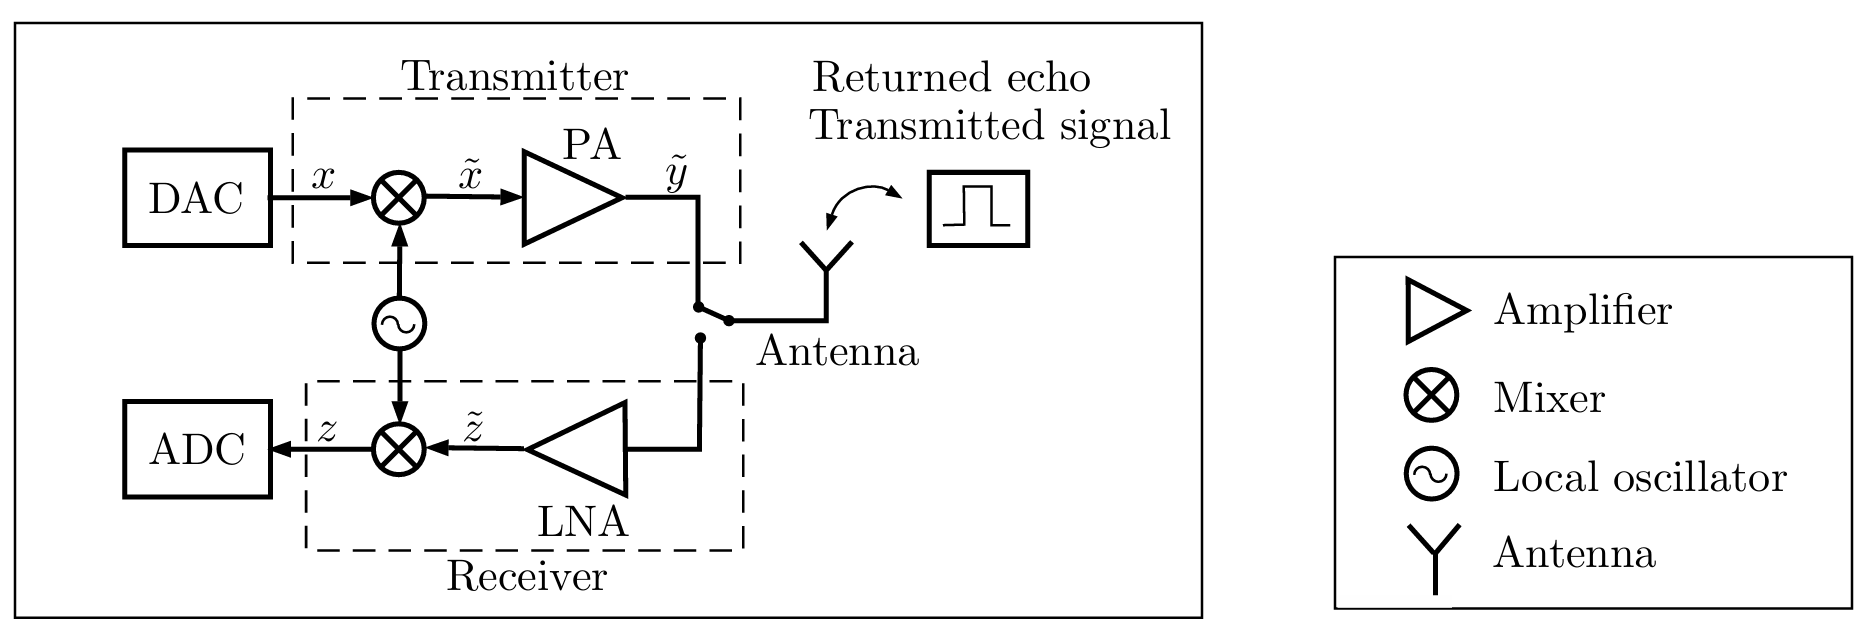
\includegraphics[width=0.9\textwidth]{Figures/Fundamentals/Radar_block_diagram}
  \caption{Simplified block diagram of pulsed radar system with explanation of symbols \cite{hanning}}
  \label{fig:radar_block_diagram}
\end{figure}

\section{Pulse Compression Radar}\label{sec:pulse_compression_radar}

A pulsed radar determines the range of a target by transmitting a pulse and measuring the round-trip delay $\tau_d$ of the returned echo \cite{pozar}. A simplified block diagram of a radar system is depicted in Figure~\ref{fig:radar_block_diagram}. An analogue baseband signal $x$ is output by the \gls{ac:dac}. The signal is subsequently upconverted to a carrier frequency by a mixer which multiplies the baseband signal with a sinusoidal signal generated by a local oscillator. The result is the \gls{ac:rf} signal $\tilde{x}$, then amplified by the power amplifier for transmission -- yielding the amplified \gls{ac:rf} signal $\tilde{y}$. Following amplification, the antenna propagates the signal in space, and if a target is present, the antenna receives the energy of a returned echo. The received signal is often weak, and thus amplified before any processing or decisions regarding detection. As the detection is noise sensitive, the amplification is handled via a \gls{ac:lna}, whose operation adds minimal noise. Before any processing and decisions whether a target is present, the signal $\tilde{z}$ is downconverted via mixing with the local oscillator and passed through an \gls{ac:adc} -- yielding the digital baseband signal $z$ \cite{skolnik}. 

As the pulse wave propagates at the speed of light $c$ in both directions (transmission and reception), the target range follows as

\begin{equation}
  R = \frac{c\,\tau_d}{2}.
  \label{eq:radar_range}
\end{equation}

Two properties govern how well this is done. The first is detection performance, which is driven by the \gls{ac:snr} at the receiver and therefore by the energy contained in the transmitted pulse -- the product of its peak power and its duration \cite{pomr}. The second is range resolution, the ability to separate two targets closely spaced in range. For a simple, unmodulated pulse of duration $\tau$, two echoes are resolved only if they are separated by at least

\begin{equation}
  \delta R = \frac{c\,\tau}{2},
  \label{eq:simple_pulse_resolution}
\end{equation}

so that resolution improves as the pulse is shortened \cite{pomr}.

Equations \eqref{eq:simple_pulse_resolution} and the energy requirement are in direct conflict for an unmodulated pulse, as both are coupled through the pulse duration $\tau$ \cite{pomr}. Lengthening the pulse raises the transmitted energy and thus the detection range, but degrades range resolution. Shortening the pulse improves resolution, but reduces the energy -- which could only be recovered by raising the peak power, and peak power is limited by what the transmitter hardware can deliver \cite{marthinmon}. Pulse compression resolves this conflict. By modulating the signal within a long pulse, the waveform bandwidth $B$ is increased independently of the pulse duration, such that $B \gg 1/\tau$ \cite{pomr}. Range resolution is then set by the bandwidth rather than the pulse duration,

\begin{equation}
  \delta R = \frac{c}{2B},
  \label{eq:range_resolution}
\end{equation}

and a long, low peak power pulse can therefore deliver the resolution of a short one.

\subsection{Linear Frequency Modulation}\label{sec:linear_frequency_modulation}

The most widely used pulse compression waveform is the \gls{ac:lfm} waveform, also known as a chirp, in which the instantaneous frequency is swept linearly across the pulse \cite{pomr}. A baseband \gls{ac:lfm} pulse is defined as

\begin{equation}
  x(t) = A\cos\left(\pi\frac{B}{\tau}t^2\right),
  \qquad -\frac{\tau}{2} \leq t \leq \frac{\tau}{2},
  \label{eq:lfm_waveform}
\end{equation}

where $A$ is the waveform amplitude, $B$ the swept bandwidth and $\tau$ the pulse duration \cite{pomr}. Differentiating the instantaneous phase gives the instantaneous frequency

\begin{equation}
  f(t) = f_0 + k\,t, \qquad k = \frac{B}{\tau},
  \label{eq:lfm_instantaneous_frequency}
\end{equation}

where $f_0$ is the carrier frequency and $k$ the frequency sweep rate \cite{marthinmon}. The linear relationship of \eqref{eq:lfm_instantaneous_frequency} is what gives the modulation its name. The sweep may be applied in either direction, producing an up-chirp or a down-chirp.

\subsection{Matched Filtering and Pulse Compression}\label{sec:matched_filtering}

The received echo is corrupted by additive noise, and the quantity that governs the probability of detection is the output \gls{ac:snr} rather than the shape of the received signal \cite{marthinmon}. The filter that maximises this output \gls{ac:snr} is the matched filter, whose impulse response is the complex conjugate of the time-reversed transmitted waveform \cite{pomr}. Applying it is equivalent to correlating the received echo against a replica of what was transmitted, and its output is the convolution

\begin{equation}
  y(t) = \int_{-\infty}^{\infty} h(\alpha)\,h^{*}(t-\alpha)\,\mathrm{d}\alpha ,
  \label{eq:matched_filter}
\end{equation}

where $h(t)$ is the impulse response of the waveform and $(\cdot)^{*}$ denotes complex conjugation \cite{marthinmon}. For the \gls{ac:lfm} waveform of \eqref{eq:lfm_waveform}, evaluating \eqref{eq:matched_filter} yields the compressed response

\begin{equation}
  y(t) = \left(1 - \frac{|t|}{\tau}\right)
         \frac{\sin\left[\left(1 - \frac{|t|}{\tau}\right)\pi B t\right]}
              {\left(1 - \frac{|t|}{\tau}\right)\pi B t},
  \qquad |t| \leq \tau ,
  \label{eq:lfm_compressed}
\end{equation}

which is the product of a triangular envelope and a term resembling a $\operatorname{sinc}$ function \cite{pomr}. For time-bandwidth products greater than roughly $20$ the response closely approximates a $\operatorname{sinc}$, whose first null lies at $t \approx \pm 1/B$ -- recovering the range resolution of \eqref{eq:range_resolution}.

The effect is therefore to concentrate the energy spread over the long transmitted pulse into a narrow, high-amplitude peak at the filter output. The degree of this concentration is quantified by the pulse compression ratio, which for an \gls{ac:lfm} waveform equals the time-bandwidth product

\begin{equation}
  \text{PCR} = \frac{\tau}{1/B} = \tau B .
  \label{eq:pulse_compression_ratio}
\end{equation}

The same product defines the pulse compression gain, the ratio of the \gls{ac:snr} at the output of the matched filter to that at its input \cite{pomr}. In modern systems, time-bandwidth products range from unity for a simple pulse to $10^6$ and beyond. It is common for the \gls{ac:snr} at the receiver input to lie below \qty{0}{\decibel}, with the signal only rising above the noise floor once the matched filter has been applied \cite{pomr}.

\subsection{Range Sidelobes}\label{sec:range_sidelobes}

Applying the matched filter to a modulated waveform produces a response consisting of a mainlobe and an accompanying sidelobe structure \cite{pomr}. The mainlobe is the portion of the response between the nulls adjacent to the peak, and its width determines the range resolution. The sidelobes, by contrast, are an undesired by-product of the modulation. They are problematic because the sidelobes of a strong target may exceed the mainlobe of a weaker one, masking its presence even when the two targets are well resolved in range \cite{pomr}.

Sidelobe performance is quantified by two metrics. The \gls{ac:psl} is the ratio of the highest sidelobe to the peak of the mainlobe, and is approximately \qty{-13.2}{\decibel} for an unweighted \gls{ac:lfm} waveform with a time-bandwidth product greater than $20$ \cite{pomr}. The \gls{ac:isl} is the ratio of the total energy contained in the sidelobes to that in the mainlobe, and is approximately \qty{-9.6}{\decibel} for the same waveform \cite{pomr}. The latter is the more relevant metric in a distributed clutter environment, where the cumulative sidelobe contributions of many resolved clutter patches add noncoherently at the range of a target.

Sidelobes are commonly suppressed by applying an amplitude weighting, such as a Taylor window, to taper the transition regions of the waveform spectrum \cite{pomr}. This constitutes a deliberate mismatch between the filter and the transmitted waveform, and consequently lowers the sidelobes at the cost of a broadened mainlobe -- and therefore degraded resolution -- along with a loss in processing gain.

Both the \gls{ac:psl} and the \gls{ac:isl} of the compressed response are used as \glspl{ac:kpi} in this thesis, as power amplifier nonlinearity distorts the transmitted waveform and consequently degrades the compressed response. The mechanisms by which this occurs are the subject of Section~\ref{sec:nonlinearity_effects}.

\section{Effects of Nonlinearity}\label{sec:nonlinearity_effects}

This section begins with a brief introduction to several concepts and equations paramount to understand nonlinearity and its effects. Firstly, a system can be called ``memoryless'' or ``static'' if its output depends solely on its current input value, and not on past input (or even output) values. Moreover, a memoryless system that is linear can be described by \cite{razavi}

\begin{equation}
  y(t) = \alpha \, x(t),
  \label{eq:memoryless_linear}
\end{equation}

where $y(t)$ is the output signal, $x(t)$ the input signal and $\alpha$ the constant gain of the system. Equation \eqref{eq:memoryless_linear} describes a linear relationship, as output is directly proportional to the input. 

On the contrary, a memoryless nonlinear system can be approximated by the power series, \cite{razavi}

\begin{equation}
  y(t) = \alpha_1 x(t) + \alpha_2 x^2(t) + \alpha_3 x^3(t) + \dotsb, 
  \label{eq:power_series}
\end{equation}

where it can be seen that the output $y(t)$ no longer shares a proportional change according to the input $x(t)$.  All electronic circuits are inherently nonlinear -- this is a fundamental truth of electronic engineering \cite{maas} -- as semiconductor materials used to build electronic components, such as transistors and diodes, do not scale their behaviour proportionally with input applied to them. The power amplifier of a transmission chain is of course not free from this truth, and existing models that attempt to describe its nonlinear behaviour are discussed in Section~\ref{sec:pa_models}. Whereas small signal operation of analogue and \gls{ac:rf} circuits can be approximated as linear, nonlinearities engender interesting effects that are not accounted for by the small-signal model. The remainder of this section elaborates on the most common phenomena observed for memoryless systems. To do so, we first describe a memoryless nonlinear system as \cite{razavi}

\begin{equation}
  y(t) \approx \alpha_1 x(t) + \alpha_2 x^2(t) + \alpha_3 x^3(t).
  \label{eq:memoryless_nonlinear}
\end{equation}

Equation \eqref{eq:memoryless_nonlinear} uses a third order polynomial; however as seen in \eqref{eq:power_series}, the power series can be extended for higher orders. The higher the order, the more precisely the equation can model the nonlinear behaviour of the system. The reader is cautioned that the effects of higher order nonlinearity terms and storage elements (introducing dynamic nonlinearity) are examined to determine whether \eqref{eq:memoryless_nonlinear} is a plausible representation \cite{razavi}. On that note, depending on operating region (bias and signal level), the degree of nonlinearity of a system can be characterised as either ``weakly'' or ``strongly'' nonlinear \cite{shi2000scs}. In practice, a power amplifier must operate well below saturation to be considered weakly nonlinear, wheareas a power amplifier operating close to the \qty{1}{\decibel} compression point (introduced in Subsection~\ref{sec:gain_compression}) is usually considered strongly nonlinear \cite{miehle}. The third order model is assumed to be a sufficient approximation for weakly nonlinear systems and is chosen for ease of instruction to explain the following effects. 

\subsection{Harmonics}

\begin{figure}[tb]
  \centering
  \begin{subfigure}[b]{0.9\textwidth}
    \centering
    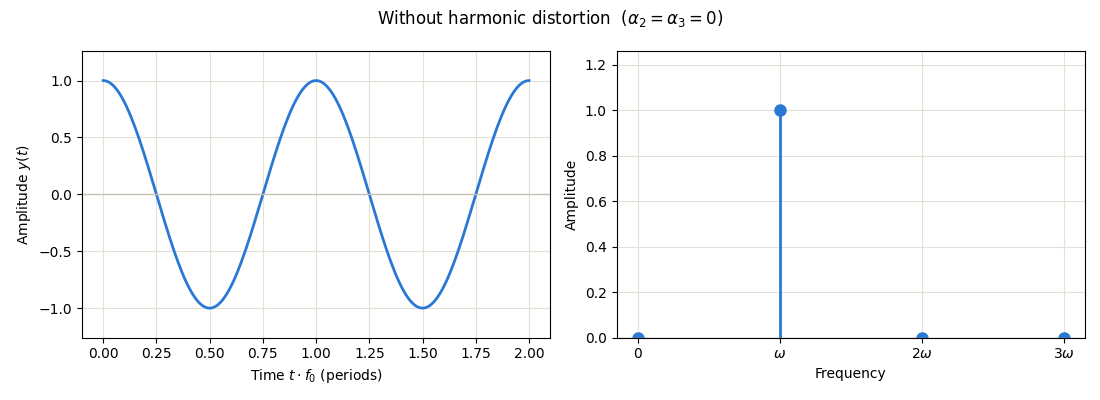
\includegraphics[width=\textwidth]{Figures/Fundamentals/Without_harmonic_distortion}
    \caption{Without harmonic distortion, i.e.\ $\alpha_2 = 0$ and $\alpha_3 = 0$.}
    \label{fig:without_harmonic_distortion}
  \end{subfigure}
  \\[\bigskipamount]
  \begin{subfigure}[b]{0.9\textwidth}
    \centering
    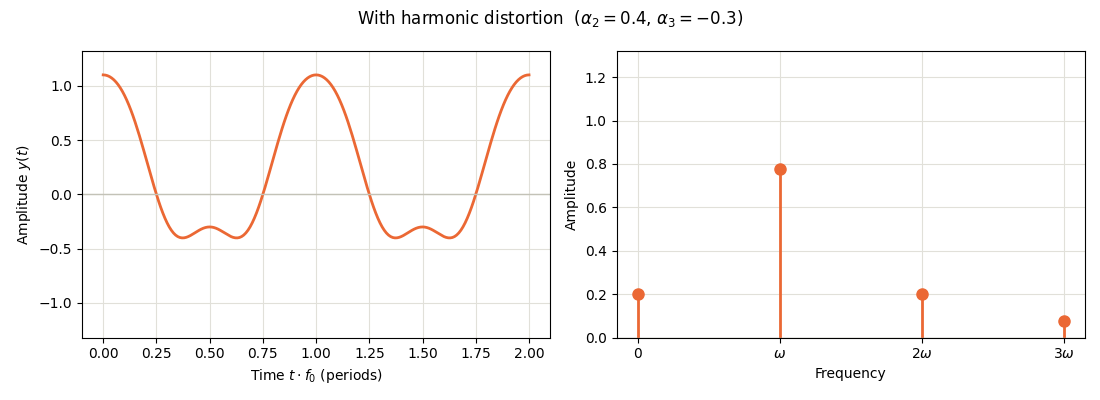
\includegraphics[width=\textwidth]{Figures/Fundamentals/With_harmonic_distortion}
    \caption{With harmonic distortion, where $\alpha_2 = 0.4$ and $\alpha_3 = -0.3$.}
    \label{fig:with_harmonic_distortion}
  \end{subfigure}
  \caption{Simulation plots of the time and frequency domain, with and without
           harmonic distortion.}
  \label{fig:harmonic_distortion}
\end{figure}

The first phenomenon is harmonic distortion. When a sinusoid is applied to a nonlinear system, the output exhibits frequency components at integer multiples of the input frequency \cite{razavi} -- these are called harmonics. To demonstrate this, we apply a sinusoidal input of $x(t) = A\cos(\omega t)$ to equation \eqref{eq:memoryless_nonlinear}, then

\begin{align}
  y(t) &= \alpha_1 A\cos\omega t + \alpha_2 A^2\cos^2\omega t
          + \alpha_3 A^3\cos^3\omega t \label{eq:harmonic_expansion} \\
       &= \alpha_1 A\cos\omega t
          + \frac{\alpha_2 A^2}{2}\left(1 + \cos 2\omega t\right)
          + \frac{\alpha_3 A^3}{4}\left(3\cos\omega t + \cos 3\omega t\right) \\
       &= \frac{\alpha_2 A^2}{2}
          + \left(\alpha_1 A + \frac{3\alpha_3 A^3}{4}\right)\cos\omega t
          + \frac{\alpha_2 A^2}{2}\cos 2\omega t
          + \frac{\alpha_3 A^3}{4}\cos 3\omega t.
          \label{eq:harmonic_terms}
\end{align}

In \eqref{eq:harmonic_terms}, the first leftmost term is a dc term. The second term is the ``fundamental'', while the second and third terms are the second and third harmonics respectively. From the above expansion, we can make several observations. Firstly, the second-oder nonlinearity produces a dc term, as the first term contains the second-order coefficient $\alpha_2$. Secondly, each order $n$ of nonlinearity generates a harmonic at frequency $n \omega$. Lastly, the amplitudes of the second and third harmonic are proportional to $A^2$ and $A^3$ respectively, hence the $n$th harmonic grows proportional to $A^n$. 

Figure~\ref{fig:harmonic_distortion} depicts the harmonic distortion visually. In the ideal linear case shown in Figure~\ref{fig:without_harmonic_distortion}, there is a single peak located at the fundamental freqeuncy $\omega$. However, the nonlinear case of Figure~\ref{fig:with_harmonic_distortion} illustrates energy being distributed to the dc term and harmonics at frequencies $2 \omega$ and $3 \omega$ -- components that are created by nonlinearity.

\subsection{Gain Compression}\label{sec:gain_compression}

\begin{figure}[tb]
  \centering
  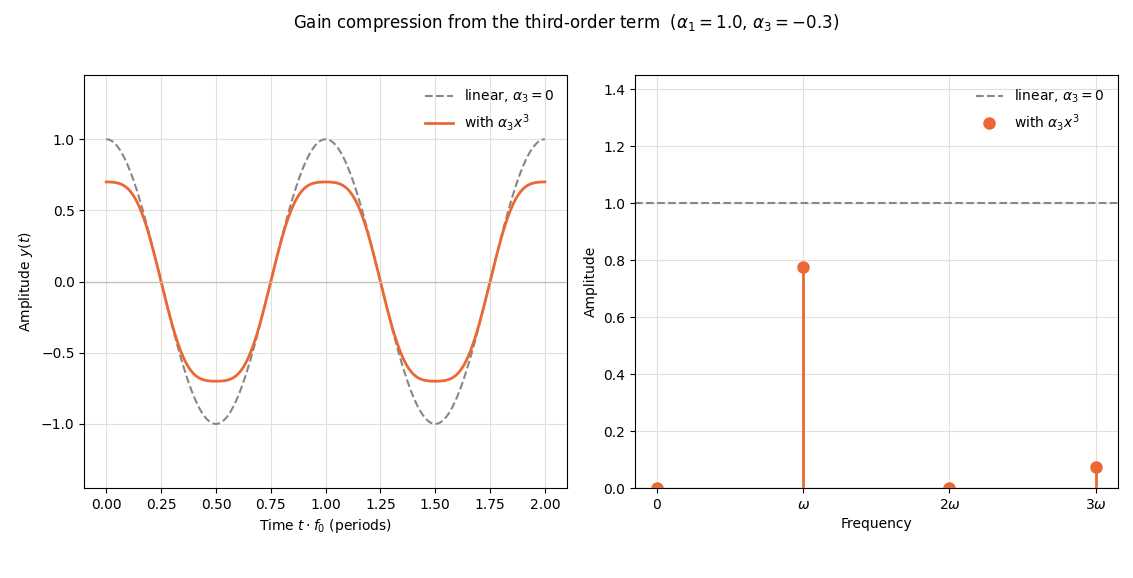
\includegraphics[width=0.9\textwidth]{Figures/Fundamentals/Gain_compression}
  \caption{Gain compression in time and frequency domain caused by third-order nonlinearity with $\alpha_3 = -0.3$}
  \label{fig:gain_compression}
\end{figure}

Another effect of nonlinearity is gain compression -- where output gain decreases with increasing input amplitude \cite{razavi}. When looking at the fundamental term in \eqref{eq:harmonic_terms}, we see that the gain experienced by $A \cos \omega t$ is equal to $\alpha_1 + \frac{3\alpha_3 A^2}{4}$. This gain is dependent on the first and third-order coefficients $\alpha_1$ and $\alpha_3$. Analytically, if $\alpha_1 \alpha_3 > 0$, then $\alpha_1 x + \alpha_3 x$ overwhelms $\alpha_2 x$ for large $x$ regardless of the sign of $\alpha_2$, leading to an ``expansive'' characteristic. Inversely, for $\alpha_1 \alpha_3 < 0$, a ``compressive'' characteristic is seen for sufficiently large $x$. Figure~\ref{fig:gain_compression} graphically demonstrates the compressive behaviour for $y(t) = \alpha_1 x(t) + \alpha_3 x^3(t)$ -- simplifying to see the effect of the third-order nonlinearity term. As before, we see a harmonic produced at $3 \omega$, but more importantly, we see the third-order term compressing the peak amplitude of the output signal in both time and frequency domain. 

\begin{figure}[tb]
  \centering
  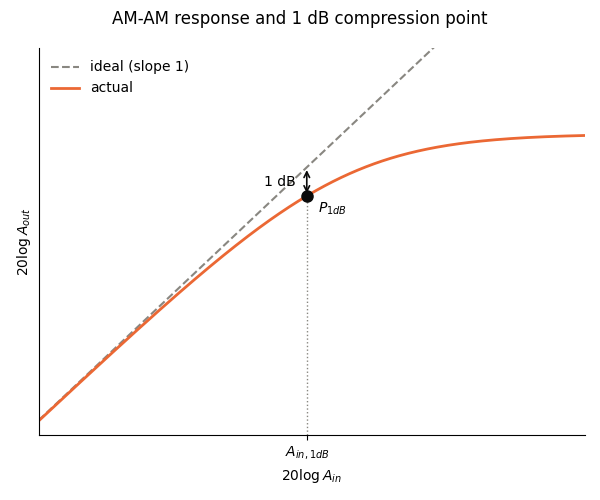
\includegraphics[width=0.9\textwidth]{Figures/Fundamentals/P1dB}
  \caption{\qty{1}{\decibel} Compression Point}
  \label{fig:P1dB}
\end{figure}

This compression is quantified by the \qty{1}{\decibel} compression point \cite{razavi}. The \qty{1}{\decibel} compression point is defined as the point where the actual output gain deviates from the ideal output gain by \qty{1}{\decibel}, typically where the output begins to near saturation. The \qty{1}{\decibel} compression point is graphically depicted in Figure~\ref{fig:P1dB}.

To obtain the \qty{1}{\decibel} compression point mathematically, we equate the compressed gain of the fundamental term, $\alpha_1 + \frac{3\alpha_3 A_{\text{in}}^2}{4}$, to \qty{1}{\decibel} less than the ideal gain, $\alpha_1$. This results in equation \eqref{eq:1db_condition}.

\begin{equation}
  20\log\left|\alpha_1 + \frac{3}{4}\alpha_3 A_{\text{in,1dB}}^2\right|
  = 20\log\left|\alpha_1\right| - \qty{1}{\decibel} .
  \label{eq:1db_condition}
\end{equation}

From \eqref{eq:1db_condition}, the \qty{1}{\decibel} compression point with reference to input amplitude is

\begin{equation}
  P_{\text{\qty{1}{\decibel}}} = A_{\text{in,1dB}} = \sqrt{0.145\left|\frac{\alpha_1}{\alpha_3}\right|} .
  \label{eq:1db_point}
\end{equation}

\subsection{Desensitisation and Blocking}

Gain compression elucidated in Subsection~\ref{sec:gain_compression} has a further side-effect of decreasing system sensitivity - called ``desensitisation'' \cite{maas}. This means that weak received signals may be blocked by strong interference signals at different frequencies. This can occur when a receiver has to process a weak signal radiated from the transmitter alongside a strong signal emitted from another nearby transmitter \cite{wambacq}. Such decrease in sensitivity from saturation is another detrimental nonlinearity effect.   

\subsection{Intermodulation}

Another highly prevalent nonlinearity effect is intermodulation. This occurs when two signals with different frequencies $\omega_1$ and $\omega_2$ are applied to a nonlinear system, where the output then exhibits frequency components that are not harmonics. This phenomenon arises from the ``mixing'' (multiplication) of the two signals \cite{razavi}. The result is components generated at the new frequencies described by \eqref{eq:new_freqs} \cite{lee}.

\begin{equation}
  \omega = m\omega_1 \pm n\omega_2.
  \label{eq:new_freqs}
\end{equation}

In \eqref{eq:new_freqs}, $\omega$ is the new frequency, where $\omega_1$ and $\omega_2$ are the original frequencies. $m$ and $n$ are positive integers including zero, and $m + n$ is equal to the order of distortion. As such, using equation \eqref{eq:memoryless_nonlinear}, we determine that the second-order nonlinearity generates intermodulation products at $\omega_1 \pm \omega_2$ and third order nonlinearity at $2\omega_1 \pm \omega_2$ and $2\omega_2 \pm \omega_1$.

To understand the generation of new components mathematically, we take a two-tone input signal $x(t) = A_1\cos \omega_1 t + A_2\cos \omega_2 t$ and apply it to \eqref{eq:memoryless_nonlinear}, resulting in

\begin{equation}
\begin{split}
  y(t) &= \alpha_1(A_1\cos\omega_1 t + A_2\cos\omega_2 t)
          + \alpha_2(A_1\cos\omega_1 t + A_2\cos\omega_2 t)^2 \\
       &\quad + \alpha_3(A_1\cos\omega_1 t + A_2\cos\omega_2 t)^3 .
\end{split}
\label{eq:two_tone_input}
\end{equation}

If we expand the right-hand side of equation \eqref{eq:two_tone_input}, and discard dc terms, harmonics and second-order components at $\omega_1 \pm \omega_2$, we obtain the third-order intermodulation products in equations \eqref{eq:im3_a} and \eqref{eq:im3_b},

\begin{align}
  \omega = 2\omega_1 \pm \omega_2 :\quad
    &\frac{3\alpha_3 A_1^2 A_2}{4}\cos(2\omega_1+\omega_2)t
     + \frac{3\alpha_3 A_1^2 A_2}{4}\cos(2\omega_1-\omega_2)t
     \label{eq:im3_a} \\
  \omega = 2\omega_2 \pm \omega_1 :\quad
    &\frac{3\alpha_3 A_1 A_2^2}{4}\cos(2\omega_2+\omega_1)t
     + \frac{3\alpha_3 A_1 A_2^2}{4}\cos(2\omega_2-\omega_1)t
     \label{eq:im3_b},
\end{align}

along with the the fundamental components of equation \eqref{eq:fundamental_components}.

\begin{align}
  \omega = \omega_1,\ \omega_2 :\quad
    &\left(\alpha_1 A_1 + \frac{3}{4}\alpha_3 A_1^3
           + \frac{3}{2}\alpha_3 A_1 A_2^2\right)\cos\omega_1 t \nonumber \\
    &+ \left(\alpha_1 A_2 + \frac{3}{4}\alpha_3 A_2^3
           + \frac{3}{2}\alpha_3 A_2 A_1^2\right)\cos\omega_2 t
     \label{eq:fundamental_components}
\end{align}

\begin{figure}[tb]
  \centering
  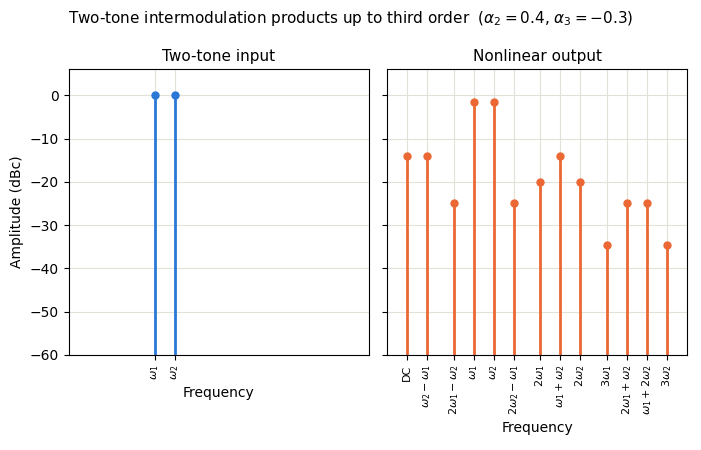
\includegraphics[width=0.9\textwidth]{Figures/Fundamentals/Two-tone_intermodulation}
  \caption{Two-tone intermodulation products up to third-order with $\alpha_2 = 0,4$ and $\alpha_3 = -0,3$}
  \label{fig:two-tone_intermodulation}
\end{figure}

\begin{figure}[tb]
  \centering
  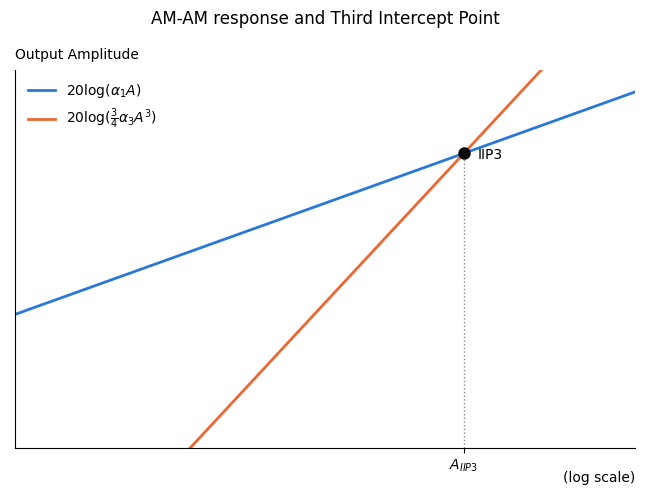
\includegraphics[width=0.9\textwidth]{Figures/Fundamentals/Third-order_intercept}
  \caption{Third Order Intercept Point}
  \label{fig:third_order_intercept}
\end{figure}

Figure~\ref{fig:two-tone_intermodulation} graphically depicts the intermodulation products. The third-order intermodulation products at $2\omega_1 - \omega_2$ and $2\omega_2 - \omega_1$ are of particular interest, as they appear directly in the vicinity of $\omega_1$ and $\omega_2$.  These corrupt the transmitted signal - often lying within the transmission bandwidth. A common measure of the extent of third-order intermodulation products is the ``third intercept point'' ($IIP_3$) \cite{razavi}. This is defined as the point where the amplitude of the intermodulation products equals that of the fundamental tones at the output. This is demonstrated graphically in Figure~\ref{fig:third_order_intercept}. In practice, this point is usually never reached, as the output typically reaches saturation before this. 

To derive the third intercept point mathematically, the amplitude of the third-order intermodulation products in \eqref{eq:im3_a} and \eqref{eq:im3_b} can first be simplified for input tones of the same amplitude, i.~e. $A = A_1 = A_2$, to $\frac{3}{4}\alpha_3 A^3$. At the input at which this theoretical input third intercept point ($IIP3$) occurs, the uncompressed linear component $\alpha_1 A$ would equal the third order intermodulation product, resulting in

\begin{equation}
  \left|\alpha_1 A_{\text{IIP3}}\right|
  = \left|\frac{3}{4}\alpha_3 A_{\text{IIP3}}^3\right|,
  \label{eq:iip3_condition}
\end{equation}

solving for $A_IIP3$ yields the input third intercept point ($IIP3$)

\begin{equation}
  A_{\text{IIP3}} = \sqrt{\frac{4}{3}\left|\frac{\alpha_1}{\alpha_3}\right|}.
  \label{eq:iip3}
\end{equation}

\subsection{Phase Distortion}\label{sec:phase_distortion}

The final effect of nonlinearity we discuss is phase distortion. Sections~\ref{sec:nonlinearity_effects} has thus far only covered effects that involves nonlinear changes to the output amplitude with respect to input amplitude. This is commonly referred to as \gls{ac:am-am} conversion. However, most power amplifier circuits exhibit memory effects due to storage components such as capacitors and inductors, resulting in phase distortion from capacitive and inductive nonlinearities. This effect is commonly referred to as \gls{ac:am-pm} conversion \cite{miehle}. The cause behind \gls{ac:am-pm} conversion can be understood by taking the fundamental component from \eqref{eq:harmonic_terms} seen in \eqref{eq:fundamental_term} \cite{maas}.

\begin{align}
  \left(\alpha_1 A + \frac{3\alpha_3 A^3}{4}\right)\cos\omega t
  \label{eq:fundamental_term}
\end{align}

The input amplitude is denoted by $A$, while $\alpha_1$ and $\alpha_3$ are the first and third order coefficients respectively. The amplitude of equation \eqref{eq:fundamental_term} consists of the first order component $\alpha_1 A$ and the third order component $\frac{3\alpha_3 A^3}{4}$. Due to nonlinear capacitance, a phase difference can exist between these two components. The response is then a vector sum of two phasors illustrated in \eqref{eq:phasor_output}.

\begin{equation}
  V = \alpha_1 A + \frac{3}{4} \alpha_3 A^3 e^{j\theta} .
  \label{eq:phasor_output}
\end{equation}

In \eqref{eq:phasor_output}, $\alpha_1$ and $\alpha_3$ are again the first and third order coefficients respectively. The sum of the phasors is denoted $V$ and the phase difference between the first (linear) and third order term is denoted by $\theta$. As such, $\frac{3}{4} \alpha_3 A^3$ possesses a different phase from the linear component. Addition of the two phasors, linear and third order, leads to a phasor $V$ with a new angle. This new angle is dependent on variations in the input amplitude $A$, regardless of whether $\theta$ remains constant \cite{maas}. Hence, changes in input amplitude result in changes in output phase of the power amplifier, namely \gls{ac:am-am} conversion. This becomes more critical as the power amplifier is driven to higher input amplitudes into saturation, because the third order component increases commensurately with $A^3$.

\section{Power Amplifier Nonlinearity Models}\label{sec:pa_models}

Section~\ref{sec:nonlinearity_effects} described the effects that nonlinearity produces, but not how the nonlinear behaviour of a particular power amplifier is captured in a form suitable for simulation. Two broad approaches exist. Physical models derive the response from the geometry, material parameters and equivalent circuit of the transistor. Such models are accurate, but they are computationally expensive and demand device knowledge that manufacturers rarely disclose. Behavioural models instead treat the power amplifier as a black box and describe only the relationship between the input and output signal envelopes \cite{schreurs}. Because this thesis is concerned with system level effects rather than device physics, and because the parameters of a behavioural model can be extracted from the limited data published in manufacturer datasheets, behavioural models are the appropriate choice and form the subject of this section.

A memoryless behavioural model is fully characterised by two functions of the input envelope amplitude. The first, $A(r)$, returns the output amplitude for a normalised input amplitude $r$ and therefore describes \gls{ac:am-am} conversion. The second, $\Phi(r)$, returns the output phase shift and describes the \gls{ac:am-pm} conversion introduced in Subsection~\ref{sec:phase_distortion}. Each model below is accordingly presented as a pair of such expressions, whose coefficients are obtained by curve fitting against measured or datasheet characteristics. It should be noted that all models presented here are memoryless, and consequently reproduce neither frequency dependent behaviour nor the long term memory effects caused by thermal and bias network dynamics.

\subsection{Saleh Model}\label{sec:saleh_model}

The earliest and most widely cited behavioural model was proposed by Saleh for \gls{ac:twta} devices \cite{saleh}. Both conversion characteristics are expressed as rational functions of the input amplitude,

\begin{align}
  A(r)    &= \frac{\alpha_a r}{1 + \beta_a r^2},        \label{eq:saleh_amam} \\
  \Phi(r) &= \frac{\alpha_\phi r^2}{1 + \beta_\phi r^2}, \label{eq:saleh_ampm}
\end{align}

where $\alpha_a$ and $\beta_a$ determine the small signal gain and the saturation level of the amplitude characteristic, while $\alpha_\phi$ and $\beta_\phi$ determine the corresponding phase characteristic. The model requires only four parameters, which is a large part of its appeal. Its shortcoming is that it was derived for travelling wave tubes, whose compression characteristic differs markedly from that of a solid state device. Consequently the Saleh model represents \gls{ac:sspa} behaviour poorly \cite{fisher}, which motivated the models that followed.

\subsection{Ghorbani and Sheikhan Model}\label{sec:ghorbani_model}

Ghorbani and Sheikhan proposed a model specifically for \glspl{ac:sspa} \cite{ghorbani}. It retains the rational structure of the Saleh model but raises the input amplitude to a fitted exponent and adds a linear term, giving

\begin{align}
  A(r)    &= \frac{x_1 r^{x_2}}{1 + x_3 r^{x_2}} + x_4 r, \label{eq:ghorbani_amam} \\
  \Phi(r) &= \frac{y_1 r^{y_2}}{1 + y_3 r^{y_2}} + y_4 r. \label{eq:ghorbani_ampm}
\end{align}

The additional exponents $x_2$ and $y_2$ allow the sharpness of the transition into compression to be adjusted independently of the saturation level, and the linear terms $x_4 r$ and $y_4 r$ correct the slope in the small signal region. The eight parameters give the model appreciably more freedom than the Saleh model, and it fits solid state devices correspondingly better \cite{fisher}. The price is that the characteristic is known to ``roll over'' beyond the fitted range, that is, the predicted output amplitude begins to decrease once the input is driven past the region covered by the fitting data. This makes the model unreliable when extrapolated into deep saturation.

\subsection{Rapp Model}\label{sec:rapp_model}

The model proposed by Rapp is the one most commonly encountered in the \gls{ac:sspa} literature \cite{rapp}. Its \gls{ac:am-am} characteristic is

\begin{equation}
  A(r) = \frac{g\,r}{\left[1 + \left(\dfrac{g\,r}{A_{\text{sat}}}\right)^{2p}\right]^{\frac{1}{2p}}},
  \label{eq:rapp_amam}
\end{equation}

where $g$ is the small signal gain, $A_{\text{sat}}$ the saturated output amplitude and $p$ the smoothness factor, which controls how abruptly the characteristic transitions from the linear region into saturation. The structure of \eqref{eq:rapp_amam} is what distinguishes the model: the output tends towards $g\,r$ for small $r$ and asymptotically towards $A_{\text{sat}}$ for large $r$, so the characteristic is monotonic and saturates gracefully by construction rather than as a consequence of the fit. As $p \rightarrow \infty$ the model approaches an ideal limiter.

Rapp provided no \gls{ac:am-pm} expression, arguing that the phase conversion of a solid state amplifier is small enough to be neglected \cite{rapp}. That assumption does not hold for the devices of interest here, and Honkanen and H\"aggman subsequently supplied a phase characteristic intended to be used alongside \eqref{eq:rapp_amam} \cite{honkanen},

\begin{equation}
  \Phi_{\text{HH}}(r) = \frac{b}{1 + e^{-c(r-a)}} \cdot \frac{1}{p_1 r + p_2},
  \label{eq:hh_ampm}
\end{equation}

in which $a$ is the cut-off input voltage at which the transistor begins to conduct, $b$ the switch-on step magnitude in degrees, $c$ the steepness of that step, and $p_1$ and $p_2$ the parameters adjusting the descending slope. The logistic first factor produces the switch-on step and the second produces the subsequent descent.

Equation \eqref{eq:hh_ampm} is strictly negative-going and bounded above by zero degrees, so it cannot represent a device whose phase shift is positive at low drive levels. Fisher and Al-Sarawi addressed this by adding an offset parameter $d$ \cite{fisher},

\begin{equation}
  \Phi_{\text{F}}(r) = \frac{b}{1 + e^{-c(r-a)}} \cdot \frac{1}{p_1 r + p_2} - d,
  \label{eq:fisher_ampm}
\end{equation}

which translates the whole characteristic vertically and thereby admits positive phase shifts. Although the coefficients of \eqref{eq:hh_ampm} were originally related to bipolar transistor parameters, the model is reported to perform well for \gls{ac:ldmos} devices also \cite{fisher}.

\subsection{Later Refinements}\label{sec:later_pa_models}

Two further refinements are relevant. White, Burr and Javornik proposed a model built from exponential terms rather than a rational function \cite{white},

\begin{align}
  A_W(r)    &= a\left(1 - e^{-br}\right) + c\,r\,e^{-dr^2}, \label{eq:white_amam} \\
  \Phi_W(r) &= \begin{cases}
                 f\left(1 - e^{-g(r-h)}\right), & r \geq h, \\
                 0,                              & r < h,
               \end{cases} \label{eq:white_ampm}
\end{align}

where $a$ and $b$ set the saturation level and the small signal gain while $c$ and $d$ adjust the shape of the characteristic within the operating region. The phase characteristic is defined piecewise, remaining zero until the threshold $h$ is exceeded.

Fisher and Al-Sarawi were unable to reproduce the published results using \eqref{eq:white_amam} and concluded that it contains a typographical error. Placing the third term inside the bracket scaled by $a$, so that

\begin{equation}
  A_{W,\text{corr}}(r) = a\left[1 - e^{-br} + c\,r\,e^{-dr^2}\right],
  \label{eq:white_corrected}
\end{equation}

recovers the accuracy originally reported \cite{fisher}. The distinction is not merely cosmetic: with \eqref{eq:white_amam} the characteristic rolls over beyond the fitted range in the manner of the Ghorbani and Sheikhan model, whereas \eqref{eq:white_corrected} behaves as expected of a solid state device. 

O'Droma, Meza and Lei proposed the modified Saleh model, developed for \gls{ac:ldmos} based amplifiers \cite{odroma}, given by

\begin{align}
  A_{MS}(r)    &= \frac{\alpha_a r^{\eta}}{\left(1 + \beta_a r^{\gamma}\right)^{\nu}} - \varepsilon,
                  \label{eq:modsaleh_amam} \\
  \Phi_{MS}(r) &= \frac{\alpha_\phi r^{\eta}}{\left(1 + \beta_\phi r^{\gamma}\right)^{\nu}} - \varepsilon.
                  \label{eq:modsaleh_ampm}
\end{align}

Comparison with \eqref{eq:saleh_amam} and \eqref{eq:saleh_ampm} shows the nature of the modification: the exponents $\eta$, $\gamma$ and $\nu$ generalise the fixed powers of the original Saleh model, and the offset $\varepsilon$ shifts the characteristic. The additional degrees of freedom let the compact rational form of the original follow a solid state device far more closely, and the model achieves the best fit of all those considered when measurement data extending into saturation is available \cite{fisher}.

\subsection{Model Comparison and Selection}\label{sec:pa_model_selection}

Fisher and Al-Sarawi compared the above models by fitting each to the same measured device data and evaluating the \gls{ac:nmse} of the resulting \gls{ac:am-am} characteristic \cite{fisher}. Their results are reproduced in Table~\ref{table:pa_model_nmse}, where a more negative figure indicates a closer fit.

\begin{table}[tb]
  \caption{\gls{ac:am-am} modelling accuracy of behavioural power amplifier models, after
           Fisher and Al-Sarawi \cite{fisher}.}
  \label{table:pa_model_nmse}
  \begin{center}
    \begin{tabular}{l|r}
      Model & \gls{ac:nmse} (\unit{\decibel}) \\
      \hline
      Saleh \cite{saleh}                        & $-27.13$ \\
      Ghorbani and Sheikhan \cite{ghorbani}     & $-35.44$ \\
      Rapp \cite{rapp}                          & $-42.33$ \\
      White et al.\ \cite{white}                & $-36.95$ \\
      White et al., corrected \cite{fisher}     & $-44.00$ \\
      Modified Saleh, O'Droma et al.\ \cite{odroma} & $-48.54$ \\
    \end{tabular}
  \end{center}
\end{table}

Two conclusions follow. Firstly, the Saleh model is clearly the weakest for solid state devices, which is consistent with its origin as a travelling wave tube model. Secondly, the ranking depends on how far the fitting data extends. When only data below saturation is available, which is the usual situation when parameters are extracted from a datasheet, the Rapp model of \eqref{eq:rapp_amam} extrapolates into the saturation region more reliably than the models that fit the measured range more tightly \cite{fisher}. When measurement data extending into saturation is available, the modified Saleh model is the most accurate in that region.

\section{Predistortion}\label{sec:predistortion}

\begin{figure}[tb]
  \centering
  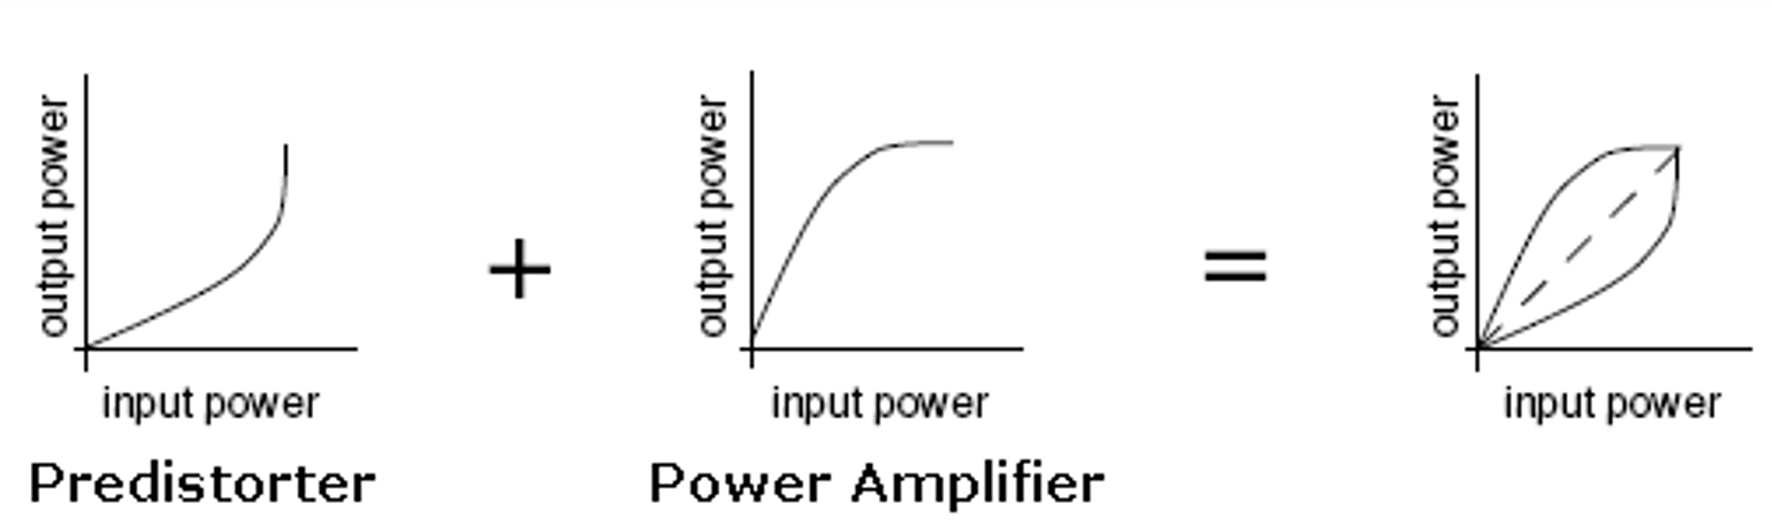
\includegraphics[width=0.9\textwidth]{Figures/Fundamentals/Predistortion_idea}
  \caption{The basic idea of predistortion \cite{marsalek}}
  \label{fig:predistortion_idea}
\end{figure}

\begin{figure}[tb]
  \centering
  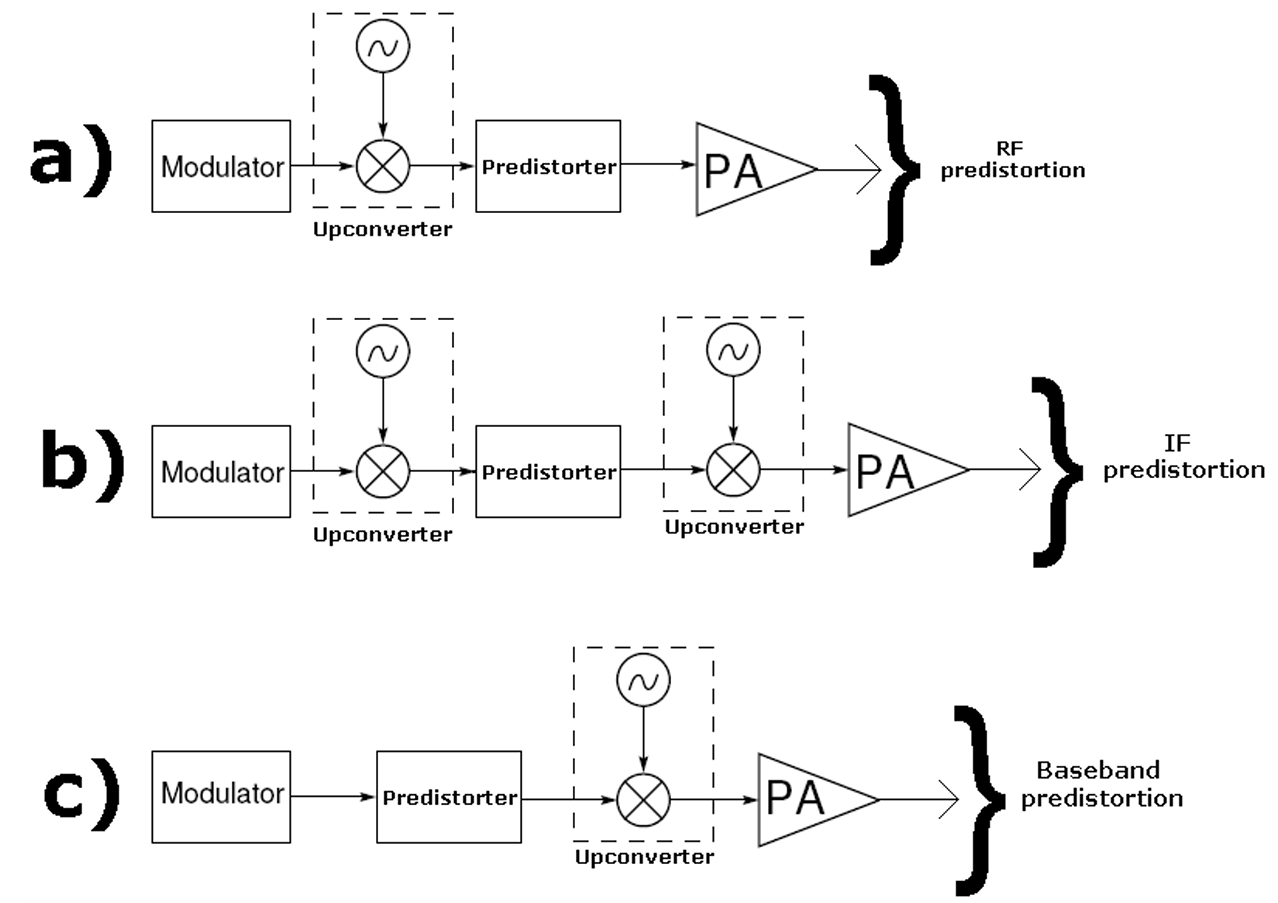
\includegraphics[width=0.9\textwidth]{Figures/Fundamentals/Predistortion_types}
  \caption{Types of predistortion: \gls{ac:rf} predistortion a), \gls{ac:if} predistortion b), baseband predistortion c) \cite{marsalek}}
  \label{fig:predistortion_types}
\end{figure}

This section introduces the concept of predistortion and the most common predistortion techniques used to mitigate nonlinearity effects. The idea of predistortion is to insert a nonlinear element (predistorter) proceeding a power amplifier, so that the cascaded transfer characteristics of the two is linear. The predistorter approximates the inverse characteristic of the power amplifier, thereby essentially cancelling out the nonlinearity at the output by first overcorrecting the input -- this underlying idea is illustrated in Figure~\ref{fig:predistortion_idea}. The result is a linear input-output relationship of the predistorter-amplifier combination. According to the position of the predistorter in the transmitter, predistortion is divided into three categories \cite{marsalek}:

\begin{itemize}
    \item \gls{ac:rf} Predistortion
    \item \gls{ac:if} Predistortion
    \item Baseband Predistortion
\end{itemize}

The position of the predistorter block for each of the three categories is depicted in Figure~\ref{fig:predistortion_types}. In \gls{ac:rf} predistortion, the predistorter element must operate at the final carrier frequency \cite{kenington}. Whereas for \gls{ac:if} predistortion, the predistorter operates at the more convenient \gls{ac:if} frequency -- allowing the predistorter block to be reused at different carrier frequencies \cite{kenington}. Finally, in baseband predistortion, the predistorter block operates at the baseband frequency, and the predistorted signal is upconverted up until the final carrier frequency. 

Power amplifier characteristics can be affected and changed by temperature changes, aging, or even output load changes \cite{durukal}. To preserve linearity for such cases, a predistorter should also adjust for this correspondingly. This divides predistortion into two further categories: ``adaptive'' and ``non-adaptive'' predistortion \cite{marsalek}. In adaptive predistortion, information on the power amplifier output is used in combination with its input signal to continually adjust the predistorter characteristic \cite{marsalek}. Adaptive predistortion can be applied to all \gls{ac:rf} predistortion, \gls{ac:if} predistortion, and baseband predistortion categories, though is most commonly seen at baseband. Such is called ``adaptive baseband predistortion'', which is a highly popular linearisation method today \cite{durukal}.

\begin{figure}[tb]
  \centering
  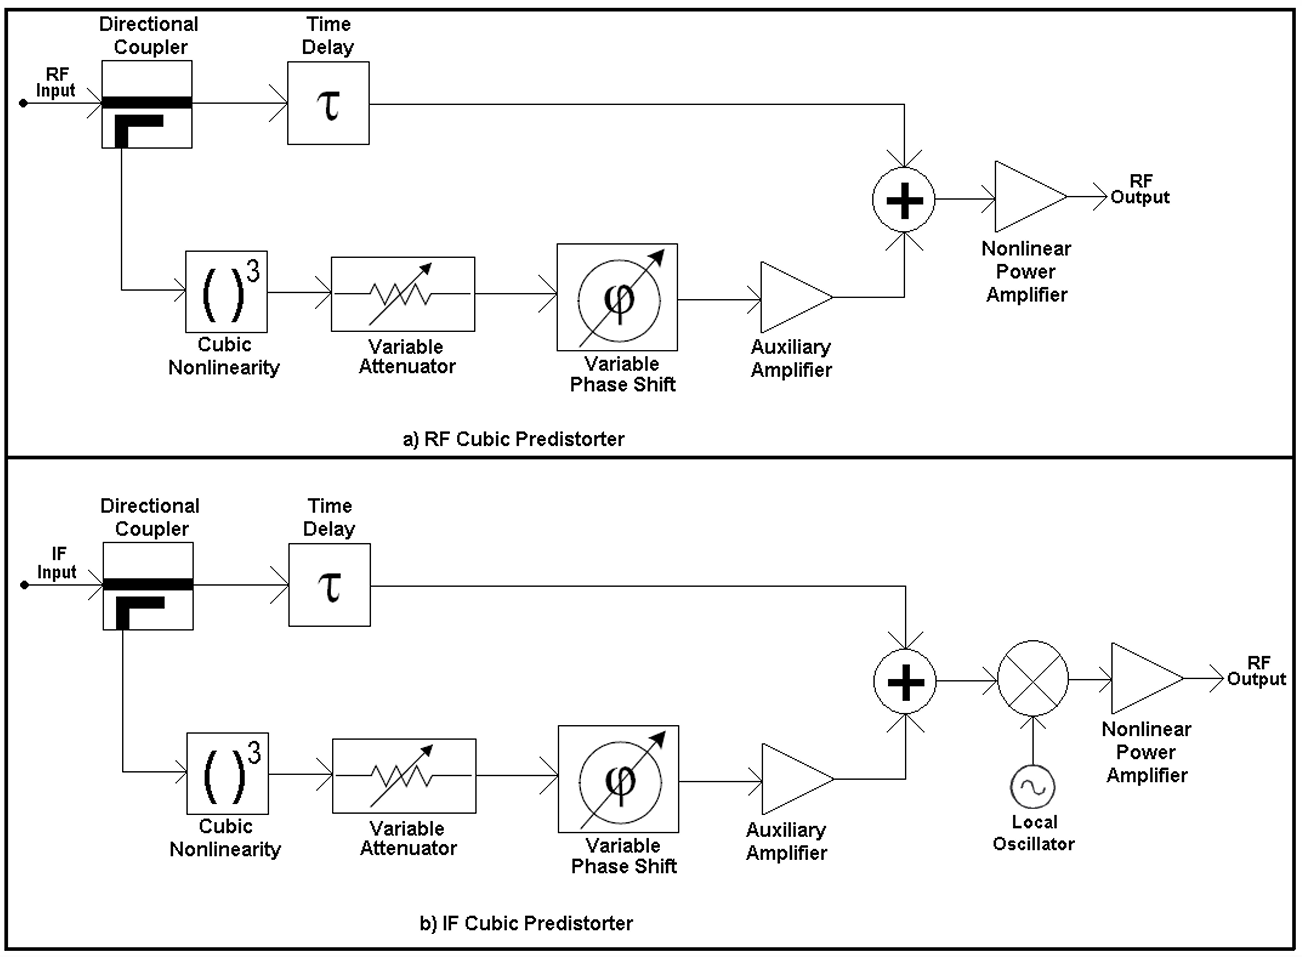
\includegraphics[width=0.9\textwidth]{Figures/Fundamentals/RF_IF_predistortion}
  \caption{a) RF cubic predistorter b) IF cubic predistorter \cite{durukal}}
  \label{fig:rf_if_predistortion}
\end{figure}

\subsection{\texorpdfstring{\gls{ac:rf}}{RF} and \texorpdfstring{\gls{ac:if}}{IF} Predistortion}

\gls{ac:rf} and \gls{ac:if} predistortion are similar in operation, differing only in the frequency at which the predistorter acts. As \gls{ac:rf} predistortion operates at the final carrier frequency, it is difficult to make adaptive, and such predistorters are consequently non-adaptive in general -- requiring the nonlinearity to be cancelled to be known in advance \cite{durukal}. Its principal advantage is its simple implementation. Operating at \gls{ac:if} instead lowers the frequency of operation, which permits the use of components that cannot work with \gls{ac:rf} signals \cite{durukal}.

The fundamental advantage of both is their ability to linearise the entire bandwidth of the amplifier, making them well suited to wideband multicarrier systems \cite{durukal, kenington}. The degree of linearity improvement attainable depends primarily on the transfer characteristic of the power amplifier itself -- the better behaved this characteristic is, the greater the improvement that can be achieved and maintained across varying input conditions \cite{kenington}.

The aim is therefore to realise a circuit whose transfer function approximates the inverse of the power amplifier characteristic, such that the combination of the two produces a linear input-output relationship. A widely used configuration for this purpose is the cubic predistorter depicted in Figure~\ref{fig:rf_if_predistortion}, which is based on the cancellation of third-order intermodulation products \cite{durukal}. The input signal is split into two paths. The upper path merely delays the signal to synchronise it with the lower path. The lower path contains a cubic nonlinearity, a variable phase shifter and attenuator, and an auxiliary amplifier. The cubic element provides a compressive characteristic, the phase shifter and attenuator adjust phase and amplitude such that the distortion cancels, and the auxiliary amplifier compensates for the considerable attenuation introduced by the cubic element -- without contributing distortion of its own, as its input power level is low \cite{durukal}.

Assuming both paths are synchronised, the upper and lower path signals are given by

\begin{align}
  v_{\text{upper}} &= a_1 v_{\text{in}}, \label{eq:cubic_upper} \\
  v_{\text{lower}} &= a_2 v_{\text{in}} - b v_{\text{in}}^3, \label{eq:cubic_lower}
\end{align}

where \eqref{eq:cubic_lower} exhibits the compressive characteristic of the cubic element. Subtracting the lower path from the upper path yields the predistorter output

\begin{equation}
  v_{\text{pd}} = \left(a_1 - a_2\right) v_{\text{in}} + b v_{\text{in}}^3 ,
  \label{eq:cubic_predistorter}
\end{equation}

which is an expansive characteristic with a linear gain of $a_1 - a_2$. By appropriate choice of $a_1$, $a_2$ and $b$, \eqref{eq:cubic_predistorter} can be used to predistort any compressive power amplifier characteristic \cite{durukal, kenington}. The cubic nonlinearity itself is commonly realised using a single diode, a pair of anti-parallel diodes, or field-effect transistors \cite{durukal}.

\subsection{Baseband Predistortion}\label{sec:baseband_predistortion}

\begin{figure}[tb]
  \centering
  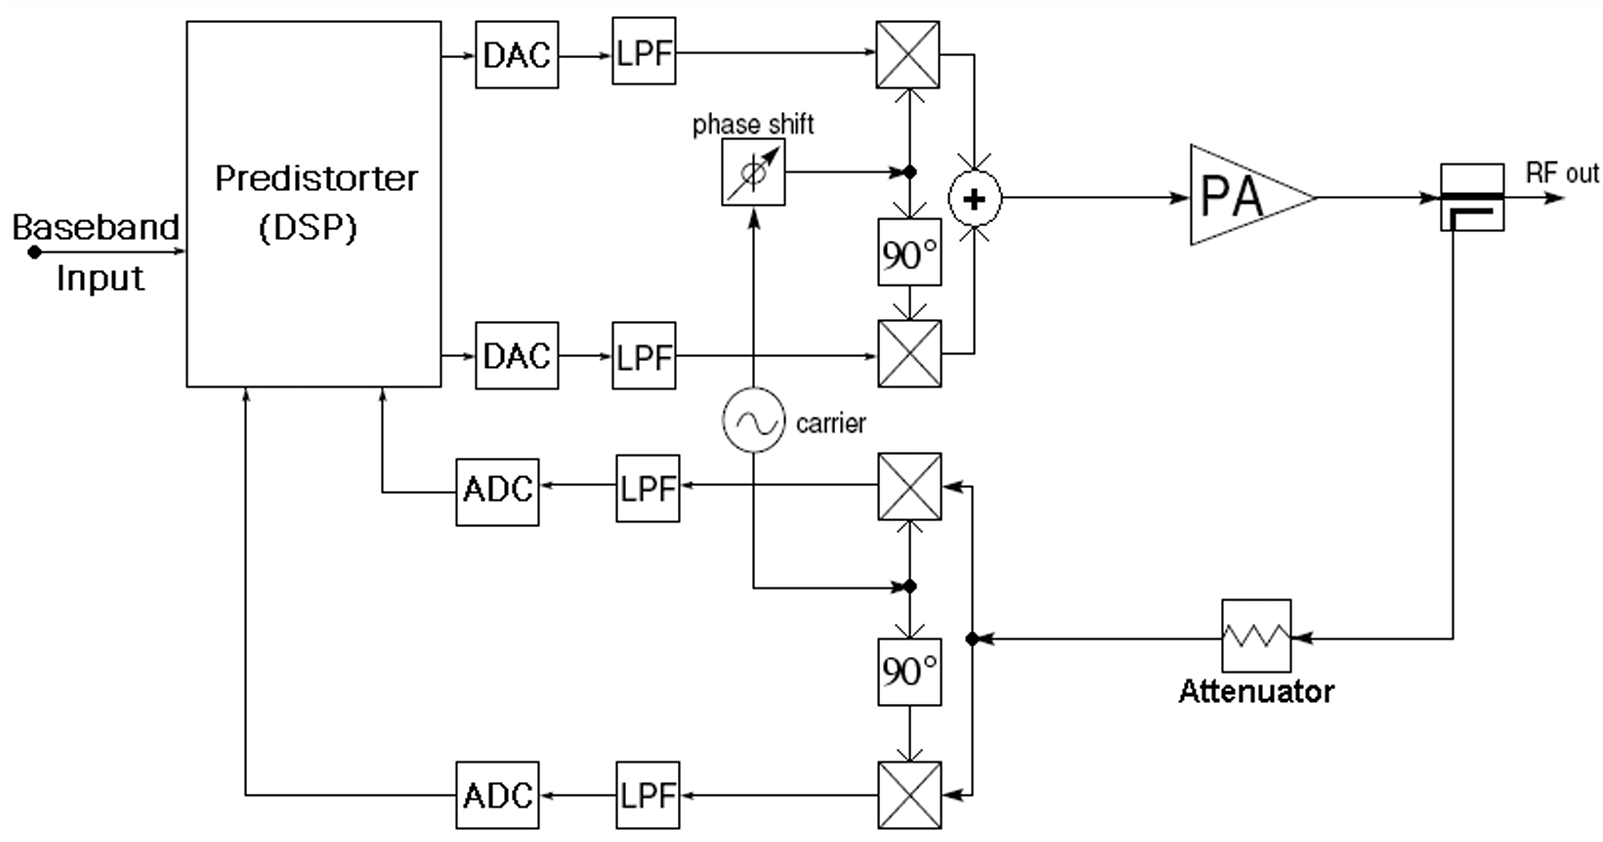
\includegraphics[width=0.9\textwidth]{Figures/Fundamentals/Adaptive_digital_bb_predistortion}
  \caption{Adaptive digital baseband predistortion \cite{marsalek}}
  \label{fig:adaptive_bb}
\end{figure}

In baseband predistortion, the predistorter element operates at baseband frequencies. This serves as an advantage, as it is significantly easier to implement the inverse characteristic of the nonlinearity at baseband due to implementation simplicity and reconfigurability. This can commonly be implemented in firmware on digital signal processing devices such as \glspl{ac:dsp}, \glspl{ac:fpga}, and \glspl{ac:asic} \cite{marsalek} -- which can be flexibly reconfigured. Thus, when the term baseband predistortion is used, it generally refers to ``digital baseband predistortion''. A further advantage of digital baseband predistortion is that it is rather straightforward to implement adaptive predistortion -- an example of this is seen in Figure~\ref{fig:adaptive_bb}. As depicted, the baseband input signal is fed into the predistorter, which outputs the predistorted digital signal. This signal is then converted by a \gls{ac:dac} to an analogue signal, then upconverted to \gls{ac:rf}, and finally amplified by the power amplifier for transmission. The adaptive nature is shown as the power amplifier output is sampled, downconverted to baseband, converted to digital form by an \gls{ac:adc}, and continuously used to adapt the predistorter characteristic \cite{marsalek}.  

\begin{figure}[tb]
  \centering
  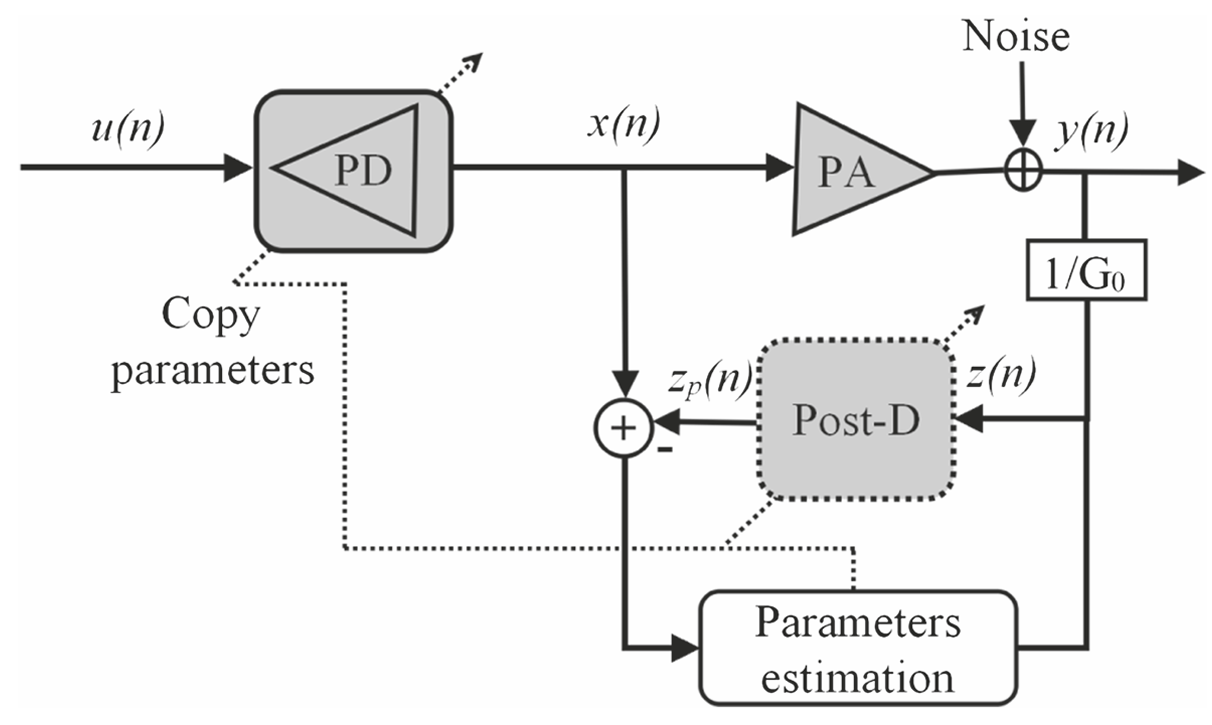
\includegraphics[width=0.9\textwidth]{Figures/Fundamentals/Indirect_learning_architecture}
  \caption{Indirect learning architecture \cite{feng2016}}
  \label{fig:ila}
\end{figure}

\begin{figure}[tb]
  \centering
  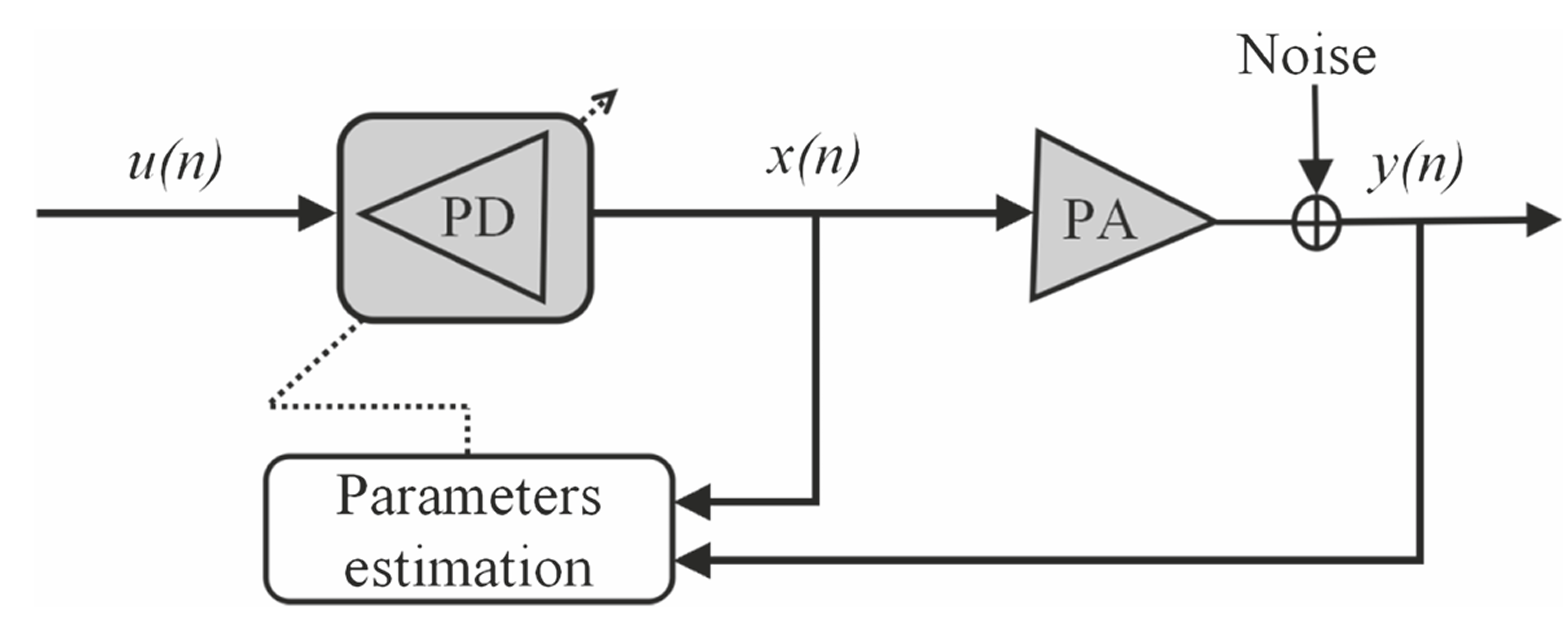
\includegraphics[width=0.9\textwidth]{Figures/Fundamentals/Direct_learning_architecture}
  \caption{Direct learning architecture \cite{feng2016}}
  \label{fig:dla}
\end{figure}

\begin{figure}[tb]
  \centering
  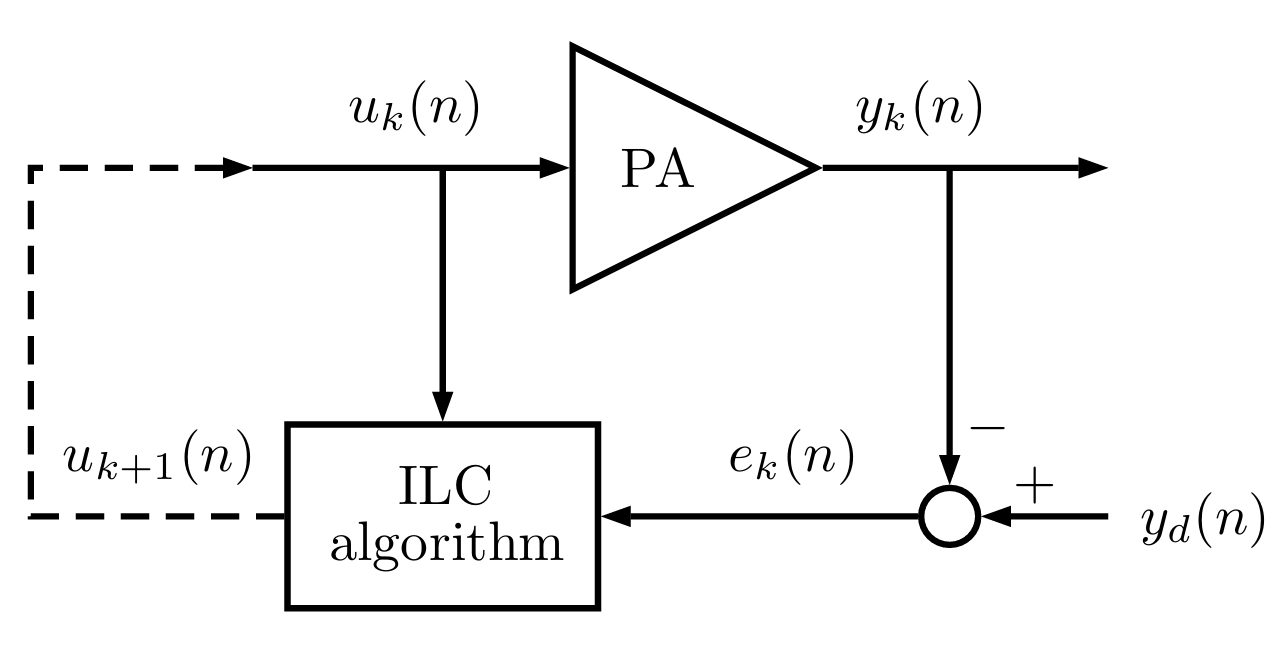
\includegraphics[width=0.9\textwidth]{Figures/Fundamentals/Iterative_learning_control}
  \caption{Iterative learning control block diagram \cite{hanning}}
  \label{fig:ilc}
\end{figure}

\begin{figure}[tb]
  \centering
  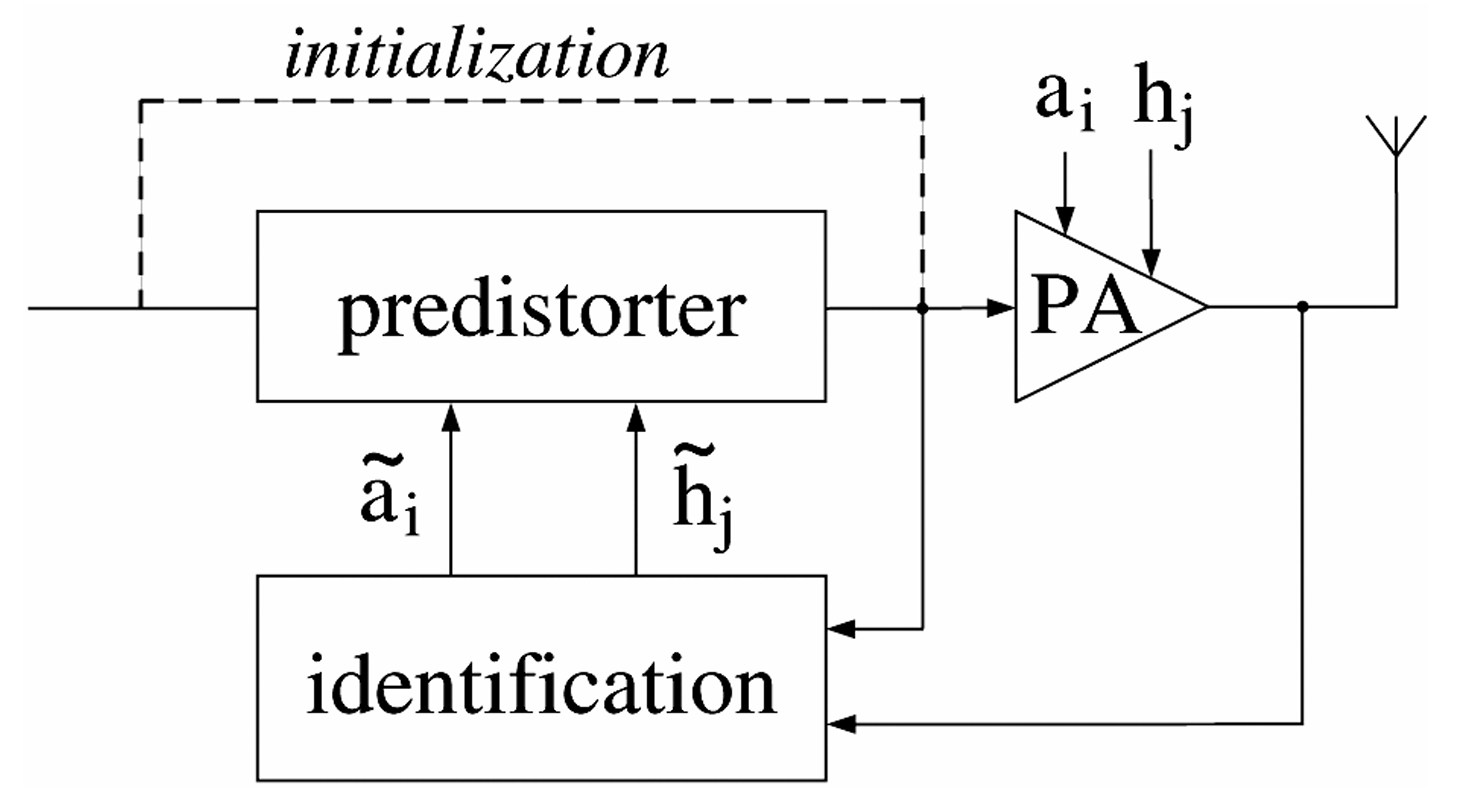
\includegraphics[width=0.9\textwidth]{Figures/Fundamentals/Adaptive_predistortion_model}
  \caption{Model of adaptive predistortion}
  \label{fig:adaptive_model}
\end{figure}

Digital baseband predistortion can be divided into the following groups. Among several techniques, digital baseband predistortion can be split into three implementation approaches -- namely \gls{ac:lut}, polynomial model, and neural network based predistorters \cite{feng2016}. Whereas neural network based predistorters can excellently approximate the nonlinear inverse characteristic, their training process is rather arduous and time consuming. Furthermore, hardware implementation is difficult in practical applications \cite{feng2016, naskas2004, mkadem2011}. \gls{ac:lut} predistorters are simple to implement, but their linearisation performance depends on the size of the \gls{ac:lut} \cite{feng2016, li2011, singla2012a, singla2012b, li2009}. Polynomial model based predistortion is also widely common -- including well known models such as the Volterra series \cite{eun1997}, model polynomial \cite{ding2004, kim2001, li2011}, generalised model polynomials \cite{morgan2006}, and etc -- with tradeoffs between different models in accuracy and computational complexity.

Digital baseband predistortion can be realised by three main learning approaches. Two of these approaches involve computing models of the power amplifier and its postinverse \cite{abihussein2012, morgan2003} -- namely \gls{ac:ila} and \gls{ac:dla}. The last approach, namely \gls{ac:ilc} \cite{chanicahuana}, aims to iteratively learn the required predistorted power amplifier input itself -- forgoing modelling of the power amplifier and its parameters. All these approaches can be implemented using the \gls{ac:lut}, polynomial model, and neural network based approaches \cite{durukal}. Both architectures have different tradeoffs. Whereas the \gls{ac:ila} is simpler by directly calculating the predistorter linearising function, the \gls{ac:dla} approach is more robust against noise at the power amplifier chain \cite{abihussein2012}. The following sections~\ref{sec:indirect_learning_architecture} and~\ref{sec:direct_learning_architecture} elaborate on the two architectures and how they each function.

\subsubsection{Indirect Learning Architecture}\label{sec:indirect_learning_architecture}

In \gls{ac:ila} \cite{ding2004}, the inverse of the power amplifier nonlinearity is first determined using the input and scaled down output of the power amplifier. This model is then forwarded to the predistorter block. This is seen in Figure~\ref{fig:ila}, where the postdistorter (Post-D) block calculates the nonlinearity inverse. The postdistorter is iteratively estimated by an identification algorithm such as the least squares method, aiming to minimise the error between power amplifier input and scaled output with each iteration. Once identified, the postdistorter block is essentially copied to the front of the power amplifier as the predistorter.

The postdistorter is commonly modelled as a memory polynomial \cite{ding2004}, whose output is given by

\begin{equation}
  z_p(n) = \sum_{k=0}^{K}\sum_{l=0}^{L} a_{kl}\,\Phi_{kl}\!\left[z(n)\right],
  \label{eq:ila_postdistorter}
\end{equation}

where $z(n) = \frac{y(n)}{G_0}$ is the scaled-down power amplifier output, $\Phi_{kl}[z(n)] = z(n-k)|z(n-k)|^{2l}$, $G_0$ the desired gain, $a_{kl}$ the complex-valued coefficients, $K$ the memory depth and $2L+1$ the highest nonlinearity order \cite{feng2016}. In a perfect system, $z_p(n) = x(n)$ is required.

Assuming a total of $N$ samples, \eqref{eq:ila_postdistorter} is expressed in matrix form as

\begin{equation}
  \mathbf{z}_p = \mathbf{Z}\mathbf{a},
  \label{eq:ila_matrix}
\end{equation}

where $\mathbf{z}_p$ collects the postdistorter output samples, $\mathbf{Z}$ the corresponding basis functions $\Phi_{kl}$ and $\mathbf{a}$ the coefficients. The latter are then extracted by the least squares method as

\begin{equation}
  \hat{\mathbf{a}} = \left(\mathbf{Z}^H\mathbf{Z}\right)^{-1}\mathbf{Z}^H\mathbf{z}_p,
  \label{eq:ila_least_squares}
\end{equation}

where $(\cdot)^H$ denotes the complex conjugate transpose operation \cite{feng2016}. Once the postdistorter model is identified, it is copied and placed in front of the power amplifier as the predistorter. 

\subsubsection{Direct Learning Architecture}\label{sec:direct_learning_architecture}

In \gls{ac:dla} \cite{kim2001, zhou2007, cottais2006}, the behaviour of the power amplifier is first modelled using its input and output. It is again estimated iteratively using the least squares method for instance. Once identified, the power amplifier model is reversed to determine the predisorter. This is depicted in Figure~\ref{fig:dla}.

The power amplifier is modelled as a memory polynomial

\begin{equation}
  y(n) = \sum_{p=0}^{P}\sum_{q=0}^{Q} c_{pq}\,\Phi_{pq}\!\left[x(n)\right],
  \label{eq:dla_pa_model}
\end{equation}

where $\Phi_{pq}[x(n)] = x(n-p)|x(n-p)|^{2q}$, $P$ is the memory depth, $2Q+1$ the highest nonlinearity order and $c_{pq}$ the model coefficients, again extracted by the least squares method \cite{feng2016}. For an ideal cascaded predistorter and power amplifier system,

\begin{equation}
  y(n) = \sum_{p=0}^{P}\sum_{q=0}^{Q} c_{pq}\,\Phi_{pq}\!\left[x(n)\right] = G_0 u(n),
  \label{eq:dla_ideal}
\end{equation}

where $u(n)$ denotes the input of the cascaded system and $x(n)$ the predistorted signal. The output is separated into a static part $s(n)$, depending only on the current input sample, and a dynamic part $d(n)$, depending on the previous input samples,

\begin{equation}
  \left\{
  \begin{aligned}
    y(n) &= s(n) + d(n) \\
    s(n) &= \sum_{q=0}^{Q} c_{0q}\,\Phi_{0q}\!\left[x(n)\right] \\
    d(n) &= \sum_{p=1}^{P}\sum_{q=0}^{Q} c_{pq}\,\Phi_{pq}\!\left[x(n)\right]
  \end{aligned}
  \right.
  \label{eq:dla_static_dynamic}
\end{equation}

From \eqref{eq:dla_ideal} and \eqref{eq:dla_static_dynamic}, the static part is rewritten as

\begin{equation}
  s(n) = e^{j\angle x(n)}\sum_{q=0}^{Q} c_{0q}\left|x(n)\right|^{2q+1} = G_0 u(n) - d(n),
  \label{eq:dla_static}
\end{equation}

where $\angle x(n)$ and $|x(n)|$ are the phase and amplitude of the predistorted signal respectively. As $d(n)$ depends only on previous samples, the right-hand side of \eqref{eq:dla_static} and the coefficients $c_{0q}$ are known at instant $n$. Taking the absolute value yields

\begin{equation}
  \left|\sum_{q=0}^{Q} c_{0q}\left|x(n)\right|^{2q+1}\right| = \left|G_0 u(n) - d(n)\right| .
  \label{eq:dla_amplitude}
\end{equation}

Equation \eqref{eq:dla_amplitude} is a high-order nonlinear equation, whose solution $|x(n)|$ is found by a root-finding procedure \cite{feng2016}. The corresponding phase is then calculated as

\begin{equation}
  \angle x(n) = \arg\left\{\frac{G_0 u(n) - d(n)}{\sum_{q=0}^{Q} c_{0q}\left|x(n)\right|^{2q+1}}\right\},
  \label{eq:dla_phase}
\end{equation}

and the predistorted signal is finally given by

\begin{equation}
  x(n) = \left|x(n)\right| e^{j\angle x(n)}.
  \label{eq:dla_predistorted}
\end{equation}

Both \gls{ac:dla} and \gls{ac:ila} approaches involve a learning phase to model characteristics -- the power amplifier for \gls{ac:dla} or postdistorter for \gls{ac:ila}. Both architectures can be made adaptive by periodically updating the power amplifier and postdistorter models respectively. This recomputes the weighting coefficients for the given memory depth and linearity order. This adaptive approach is illustrated in Figure~\ref{fig:adaptive_model}, where the $a$ and $h$ coefficients represent nonlinearity and memory depth respectively.

Whereas the \gls{ac:ila} approach is generally easier to implement than \gls{ac:dla} due to its direct derivation of the nonlinear inverse characteristic, \gls{ac:dla} is more robust in the presence of noise \cite{abihussein2012}. However, this does not matter in the context of pulse compression radar. This is because the same set of waveforms is transmitted. As every pulse is identical, the power amplifier output can be captured for many pulses and averaged; hence, the random noise averages out. 

On that note, the \gls{ac:dla} and \gls{ac:ila} algorithms are further simplified for pulse compression radar, as the predistorted signal $x(n)$ only needs to be computed once for a recurring pulse. It can be stored and loaded for transmission, saving the computational time and workload of having to recalculate $x(n)$ for the case of varying inputs.  

\subsubsection{Iterative Learning Control}\label{sec:iterative_learning_control}

\gls{ac:ilc} is a control theory technique to iteratively learn the power amplifier input that minimises the difference between its output and the desired reference signal \cite{chanicahuana}. This is a non-model based learning approach which aims to directly find the optimal input signal to the power amplifier, serving as the predistorted signal. The derived optimal predistorted signal can also then be used a reference to extract power amplifier and predistortion modelling parameters, though the approach itself does not model the power amplifier nor predistortion. Rather, it aims to iteratively minimise the error between the power amplifier output and its theoretical ideal linear output. As such, the \gls{ac:ilc} algorithm requires that the desired output response is the same for each iteration, which is suitable for pulse compression radar \cite{hanning}. The learned optimal input signal is stored and used directly as the predistorted signal, forgoing the need for a predistorter structure. 

A block diagram of the \gls{ac:ilc} algorithm is depicted in Figure~\ref{fig:ilc}. $u_k(n)$ and $y_k(n)$ are the input and output signal of the power amplifier respectively for iteration $k$. $y_d(n)$ is the desired ideal unamplified linear output of the power amplifier. The algorithm starts by initialising both $u_1(n)$ (the first iteration) and $y_d(n)$ to the reference input signal $x(n)$ i.~e. $u_1(n) = x(n)$ and $y_d(n) = x(n)$. Then, for iterations $k = 1$ to $K$, the following steps are performed \cite{chanicahuana}: Firstly, $u_k(n)$ is fed into the power amplifier. The output $y_k(n)$ is correspondingly captured. Then, the difference between the scaled-down captured output and desired reference output is calculated as the error $e_k(n) = y_d(n) - \frac{y_k(n)}{G}$ where $G$ is the power amplifier gain. The error signal $e_k(n)$ is then used to update the input of the next iteration $u_{k+1}(n) = u_k(n) + e_k(n)$. With each iteration, the error decreases until an optimal predistorted power amplifier input signal is obtained. 

The \gls{ac:ilc} approach is ideal for pulse compression radar, as the same set of pulse signals is transmitted. The optimal predistorted waveform for these pulses simply needs to be learned and stored by applying \gls{ac:ilc}, to then be easily loaded for transmission. The algorithm is made adaptive by periodic recomputation of the optimal waveform in the background.



	\input{Chapters/Requirements}
	...
}
\Appendix{
	\chapter{Appendix}
\label{appendix}

%*********************************************************************************
%---------------------------------------------------------------------------------
\section{Test Series}
%---------------------------------------------------------------------------------
%*********************************************************************************

...

	...
}
\end{lstlisting}

%*********************************************************************************
%---------------------------------------------------------------------------------
\section{Specific Files}
%---------------------------------------------------------------------------------
%*********************************************************************************

Apart from \emph{Thesis.tex} there are only few provided files that you should or must modify. Let's have a look.

%---------------------------------------------------------------------------------

\paragraph{Additional packages} The file \emph{.$\backslash$Preamble$\backslash$Packages.tex} contains frequently used packages (e.~g. math, listings, TikZ drawings). This is a great place to add further required packages, isn't it?

%---------------------------------------------------------------------------------

\paragraph{Bibliography} Add literature to \emph{.$\backslash$SpecialPages$\backslash$Bibliography.bib}. The file contains sample BibTeX entries for theses~\cite{Lassahn24}, books~\cite{Burger15,Chollet26}, and articles~\cite{HenselVogel25}. For further entry types and additional information refer to, for instance, the related Wikipedia article\footnote{\url{https://de.wikipedia.org/wiki/BibTeX} (Accessed: 15.09.2026)}.

Please note that a bibliography should contain only sources that are not subject to potential changes (e.~g., books, manuals, theses, ISO standards). Other sources -- in particular online resources such as the Wikipedia article referred to in the previous paragraph -- should be referenced using a footnote with url and the date of access.
%
\begin{lstlisting}[language=bash]
HAW Hamburg\footnote{\url{www.haw-hamburg.de} (Accessed: 15.09.2026)}
\end{lstlisting}

%---------------------------------------------------------------------------------

\paragraph{Use of AI tools} Be aware that you \emph{must} declare all use of AI tools in the declaration on page~\pageref{Declaration:AI}. Modify the table in \emph{.$\backslash$SpecialPages$\backslash$DeclarationOnUseOfAI.tex} accordingly.

%*********************************************************************************
%---------------------------------------------------------------------------------
\section{Online and Local Editors}
%---------------------------------------------------------------------------------
%*********************************************************************************

The prior sections served the purpose to clarify how to use the template. In the following, let's briefly discuss online and local editors. We recommend using a local \LaTeX\ environment, which is easy to set up, easy to use, works without internet connection, and does not introduce risks with respect to the protection of confidential data.

%---------------------------------------------------------------------------------

\paragraph{Overleaf} Many students seem to use the online editor Overleaf\footnote{\url{https://www.overleaf.com} (Accessed: 15.09.2026)} to work on their written thesis. To create your project, choose \emph{Existing project (.zip)} and select or drag and drop the provided zip file of this template. Note that in our tests the compilation process frequently ran into timeout errors. The cause is not fully understood yet, however, following workaround typically solved the issue during our tests:
%
\begin{enumerate}
	\item Change the language to German (\emph{DE}) in \emph{Thesis.tex}.
	\item Do any modification in \emph{.$\backslash$Preamble$\backslash$Packages.tex} (e.~g., change a comment and change it back to its original text).
	\item Press the red button \emph{Clear cached files} in the lower right of the window.
	\item Select \emph{Recompile from scratch} from the drop-down menu next to the green button \emph{Recompile}.
	\item If necessary, press \emph{Recompile} several times until the PDF is generated. Once compilation is successful, you may change the language back to English.
\end{enumerate}
%
Alternatively, use a local installation where in our experience such issues do not exist.

%---------------------------------------------------------------------------------

\paragraph{Local environments} Instead of using an online editor, you should consider working with a local \LaTeX\ environment. This approach brings only little initial effort and has some advantages (e.~g., protection of confidential data). While there are different software packages available, in my experience it is comfortable to first install MiKTeX\footnote{\url{https://miktex.org/} (Accessed: 15.09.2026)} as \TeX\ distribution and use TeXstudio\footnote{\url{https://texstudio.org/} (Accessed: 22.09.2026)} as editor. There is no need to create a project. Instead, open the main file \emph{Thesis.tex} to start editing (Fig.~\ref{Fig:Introduction:TeXstudio}).%
%
\begin{figure}[t]
	\centering
	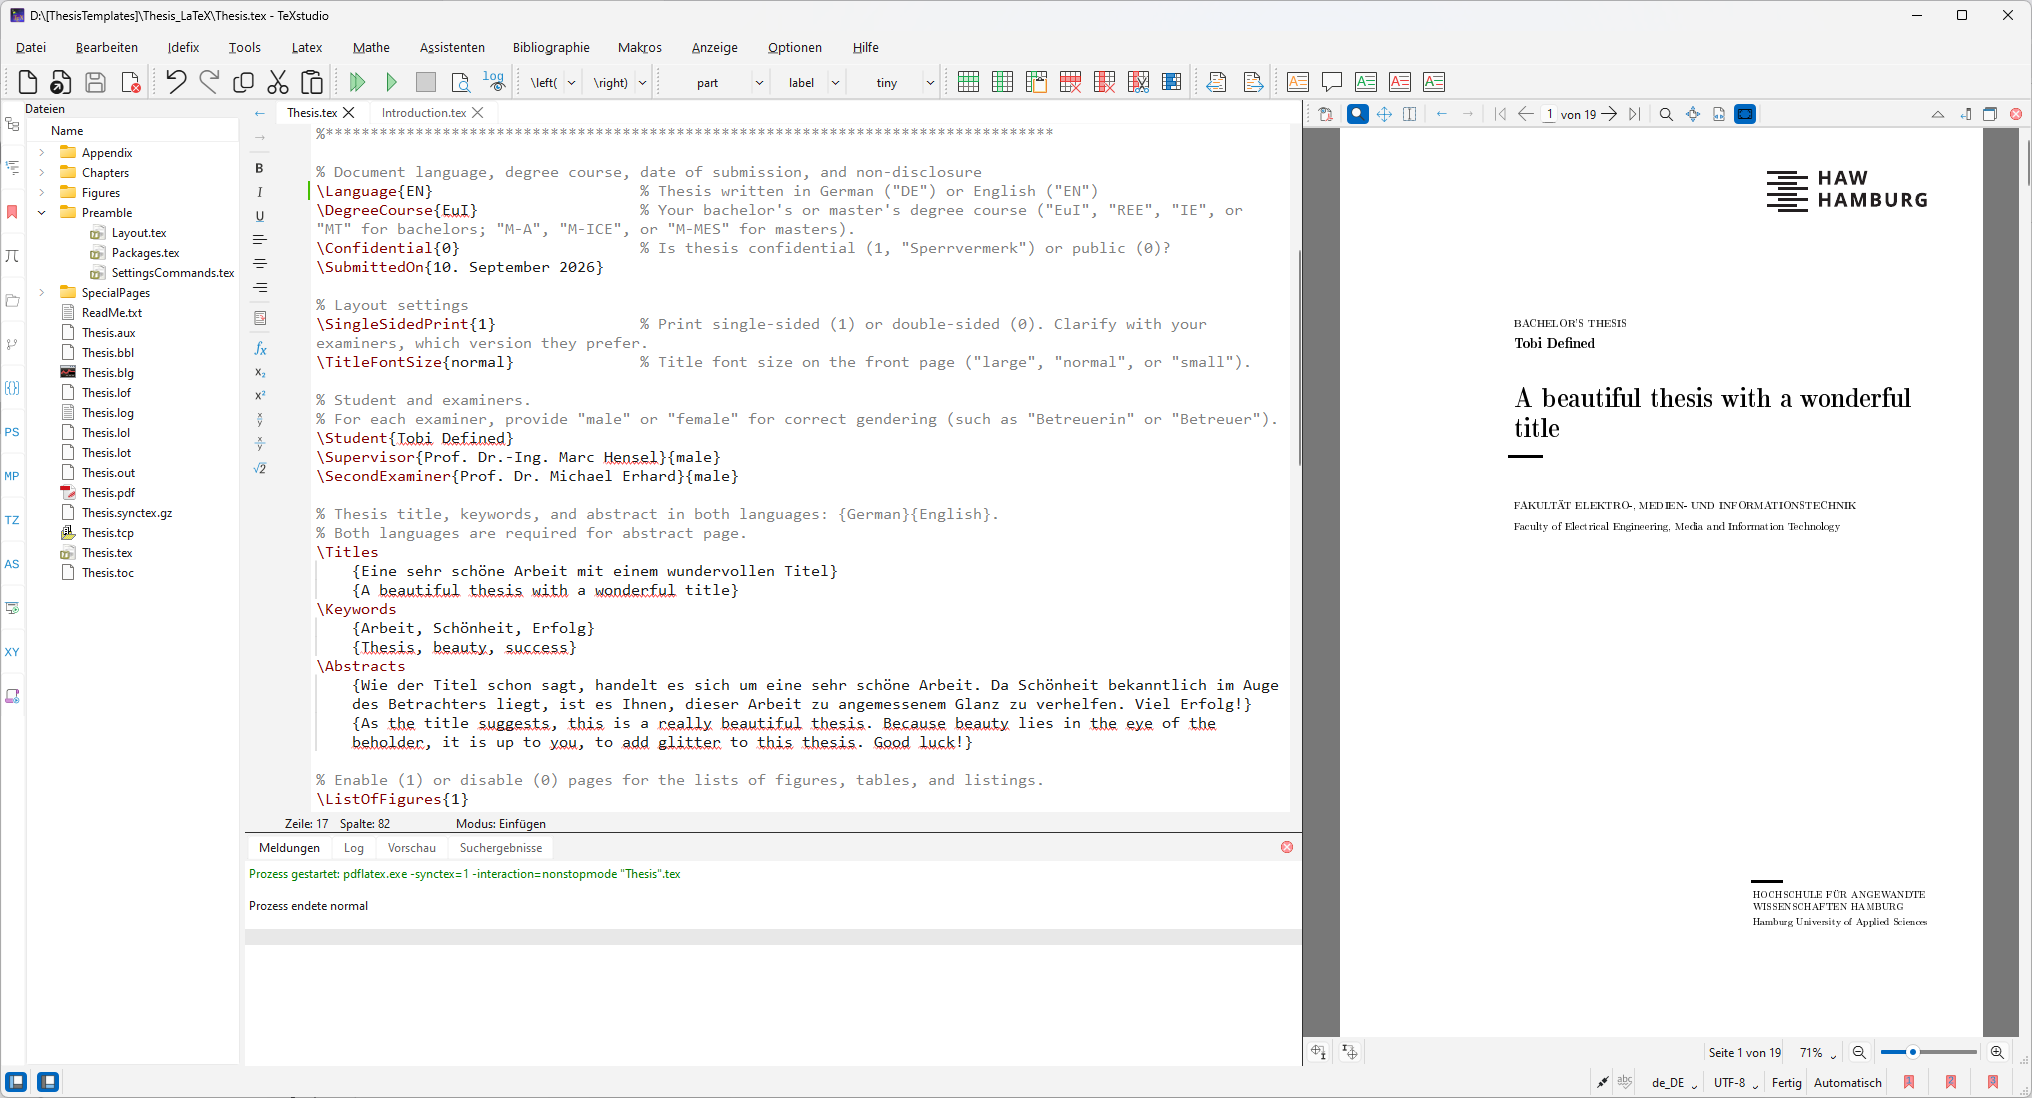
\includegraphics[width=\textwidth]{Figures/Introduction/TeXstudio}
	\caption{\LaTeX\ editor TeXstudio}
	\label{Fig:Introduction:TeXstudio}
\end{figure}
%
A good alternative is the editor TeXnicCenter\footnote{\url{https://www.texniccenter.org/} (Accessed: 15.09.2026)} (Fig.~\ref{Fig:Introduction:TeXnicCenter}), which requires initial configuration.
%
\begin{figure}[t]
	\centering
	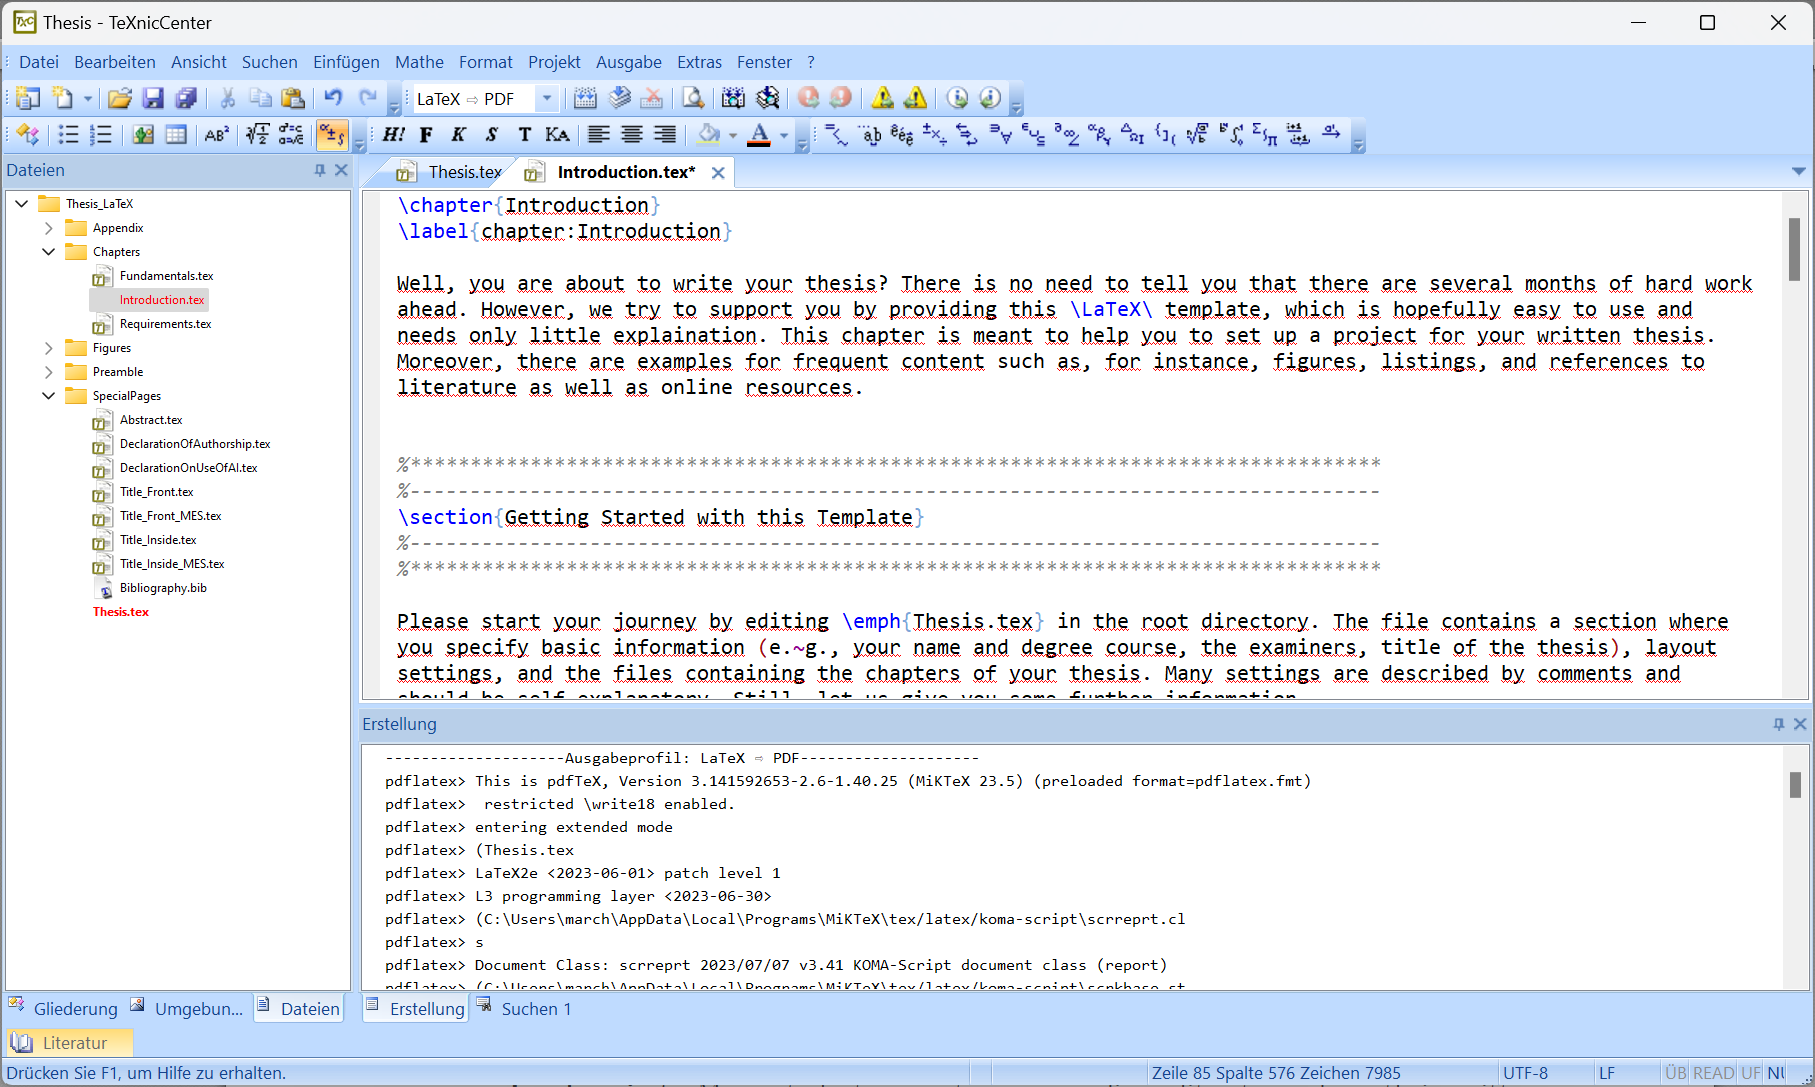
\includegraphics[width=\textwidth]{Figures/Introduction/TeXnicCenter}
	\caption{\LaTeX\ editor TeXnicCenter}
	\label{Fig:Introduction:TeXnicCenter}
\end{figure}

%*********************************************************************************
%---------------------------------------------------------------------------------
\section{Figures, Tables, and Listings}
%---------------------------------------------------------------------------------
%*********************************************************************************

Finally, let's take advantage of the fact that the \LaTeX\ sources of this document are available to you. This gives us the opportunity to provide examples how to include, for instance, figures, tables, and listings in your thesis.

%---------------------------------------------------------------------------------

\paragraph{Figures and tables} Naturally, the following is a recommendation, not a strict rule. However, it is good practice to position figures and tables at the top of a page with the text passages below (e.~g., Figures~\ref{Fig:Introduction:TeXstudio} and \ref{Fig:Introduction:TeXnicCenter}, Table~\ref{Tab:Introduction:SelectedCommands}).
%
\begin{table}[t]
	\centering
	\small
	\caption{Selected template commands}
	\begin{tabular}{ll} \toprule
		\textbf{Command} & \textbf{Valid values} \\ \toprule
		Language & DE, EN \\ \midrule
		SingleSidedPrint & 0, 1\\ \midrule
		TitleFontSize & large, normal, small\\ \bottomrule
	\end{tabular}
	\label{Tab:Introduction:SelectedCommands}
\end{table}
%
To achive this layout, pass the option \emph{t} to the environment of the figure or table, for instance:
%
\begin{lstlisting}
\begin{figure}[t]
	...
\end{figure}
\end{lstlisting}

%---------------------------------------------------------------------------------

\paragraph{Listings} The \emph{listings} package provides support for source codes. In particular, use the environment \emph{lstlisting} to generate code within the running text
%
\begin{lstlisting}
int sum = 0;
\end{lstlisting}
%
as well as numbered listings like Listing~\ref{Listing:Introduction:OpenImage}.
%
\begin{lstlisting}[float=t,frame=t,captionpos=b,caption={Open and display an image},label={Listing:Introduction:OpenImage}]
int main()
{
	cv::Mat image = cv::imread("D:/Docks.jpg", cv::IMREAD_ANYCOLOR);
	cv::imshow("Image", image);
	cv::waitKey(0);
	return 0;
}
\end{lstlisting}
%
To customize the layout, such as color schemes, line numbers, language-dependent syntax highlighting, and so on, please refer to the appropriate section of the file \emph{.$\backslash$Preamble$\backslash$Packages.tex} and the documentation\footnote{\url{https://ctan.org/pkg/listings} (Accessed: 15.09.2026)} of the package.

